\documentclass[a4paper,10pt]{report}

\usepackage[utf8]{inputenc}  
\usepackage[T1]{fontenc}
\usepackage{graphicx}
\usepackage{tikz}
\usepackage[top=2cm, bottom=2cm, left=2cm, right=2cm]{geometry}
\usepackage{hyperref}
\usepackage{multicol}
\usepackage{multirow}
\usepackage{caption}
\usepackage{rotating}
\usepackage{colortbl}

\usepackage{float}
\graphicspath{{pictures/}}
\DeclareUnicodeCharacter{00A0}{ }
\widowpenalty=10000
\clubpenalty=10000


\setlength{\parindent}{0.5cm}
\begin{document}
\title{Projet Imagerie Multispectrale}
\author{Aurélien Barbotin Pierre David Benjamin Michelland Youna le Vaou}

\maketitle

\chapter{Présentation du projet}
%opening

\section{Contexte}

Ce projet s'inscrit dans le cadre de notre formation ingénieur. Il s'étend sur six semaines et a été encadré par M. Brodu, chercheur post-doctorant à l'Inria dans l'équipe GeoStat (Géométrie et Statistiques dans les données d'acquisition) à Bordeaux. 

\subsection{Enjeux de la surveillance satellite}

Ce projet se situe dans un domaine particulier de l'utilisation des satellites orbitant autour de la Terre : la classification et le suivi des sols. 
Les applications concernent aussi bien l'agriculture que la surveillance environnementale (fonte des glaces, observation des océans et des forêts) en passant par la géologie, sans oublier la cartographie.

De manière plus concrète, M. Brodu, notre encadrant pédagogique, a mené des projets de traitement d'image satellite pour la surveillance environnementale. Il a notamment travaillé avec l'équipe OptIC (Optimal Inference in Complex and Turbulent Data), associée à l'Inria. L'idée était de suivre l'évolution de la végétation afin de repérer les zones de sécheresse, et ainsi pouvoir mieux gérer les ressources en eau. Une classification des sols de la région autour de Roorkee (Inde) a ainsi été effectuée. 
Cette classification a été réalisée grâce à des données d'imagerie multispectrale, qui est une technique de télédétection. C'est donc à cette technique que nous nous sommes intéressés, même s'il en existe d'autres (imagerie radar par exemple). 

\subsection{Imagerie satellite multispectrale}

Une image photographique couleur "classique" contient en réalité trois images : l'une dans le rouge, l'autre dans le vert et la troisième dans le bleu (RGB en anglais ou RVB en français). Elle ne contient donc que des informations dans le visible. 
\begin{figure}[H]
  \centering
    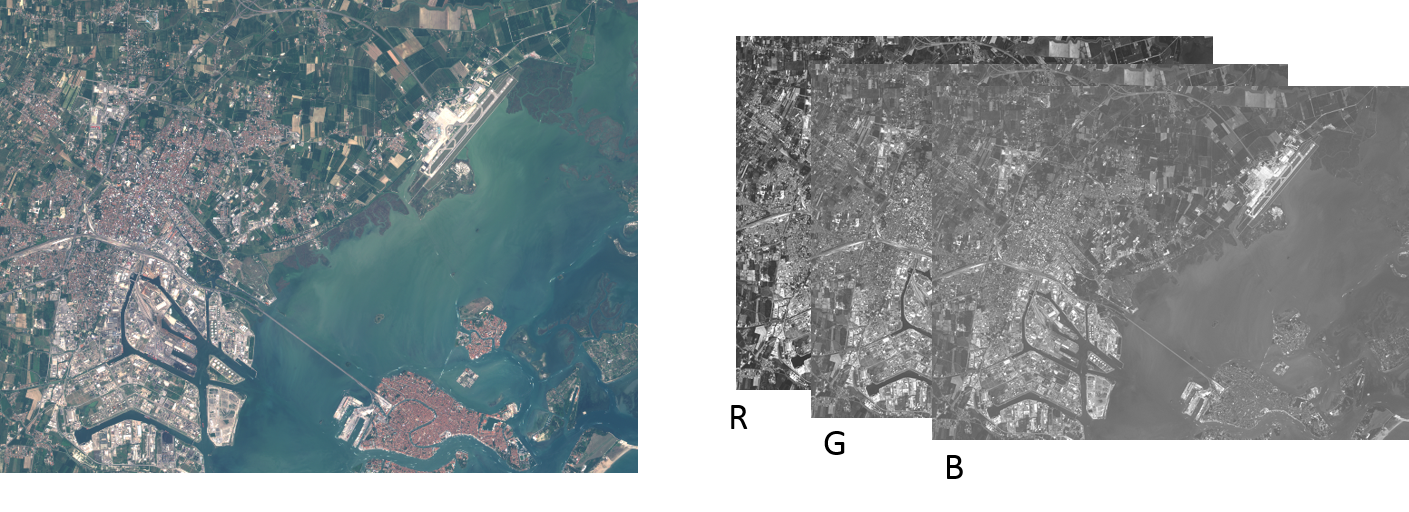
\includegraphics[width=0.75\textwidth]{veniseRGB}
  \caption{Image RGB du Nord de l'Italie (près de Venise)}
  \label{fig:veniseRGB}
\end{figure}

Une image multispectrale, quant à elle, est formée de nombreuses images prises à des longueurs d'ondes variées. Elle contient donc plus d'informations, et selon les longueurs d'ondes d'acquisition peut avoir, en plus du visible, des informations dans l'ultraviolet ou l'infrarouge.

\begin{figure}[H]
  \centering
    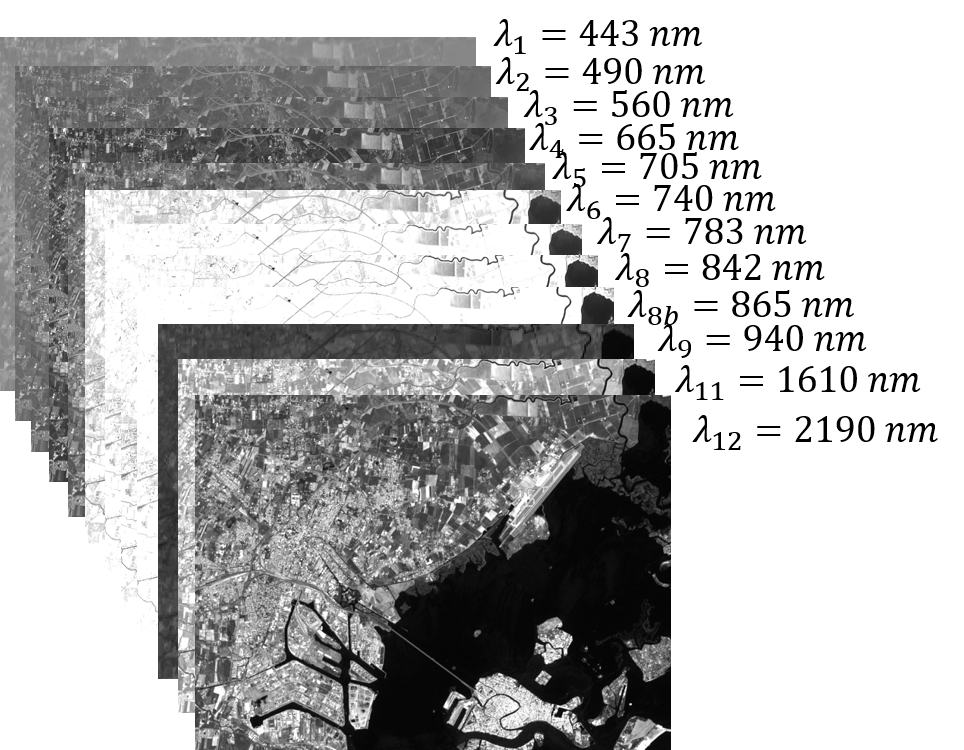
\includegraphics[width=0.5\textwidth]{multispectrale.png}
  \caption{Image multispectrale du Nord de l'Italie (près de Venise)}
  \label{fig:veniseMulti}
\end{figure}

Parmi les satellites utilisant cette technologie on trouve les satellites Aqua et Terra MODIS (Moderate-Resolution Imaging SpectroRadiometer). Ces deux satellites, lancés par la NASA en 1999 et 2002, imagent l'intégralité de la surface de la Terre tous les deux jours. Les données sont ensuite traitées et mises à disposition du public gratuitement, ce qui en a fait une des principales sources d'images satellites multispectrales. Ces satellites sont capables de mesurer 36 bandes fréquentielles avec trois résolutions différentes : 250m, 500m et 1000m par pixel\cite{nasa}. L'objectif de cette mission est de "jouer un rôle vital dans le développement de modèles globaux, validés et interactifs de systèmes terrestres capables de prévoir des changements globaux avec suffisamment de précision pour aider les décideurs politiques à prendre des décisions avisées concernant la protection de notre environnement."

La faible résolution des données MODIS ne permet en revanche pas de discerner des détails comme des cours d'eau ou des habitations, et des données plus précises sont donc nécessaires pour obtenir de meilleures classifications. 

Dans le cadre du projet \textit{Copernicus} d'observation de la Terre, l'agence spatiale européenne (ESA) développe en ce moment les missions Sentinel. Chacune de ces missions consiste en une paire de satellites en orbite autour de notre planète, récoltant des données sur la surface et l'atmosphère. Ainsi, les satellites Sentinel 2 (Sentinel 2-A lancé le 23 juin 2015 et 2-B dont le lancement est prévu pour la seconde moitié de 2016)\cite{sent2} récoltent des données multispectrales sur 13 bandes de fréquence : 4 bandes avec une résolution de 10m/pixel, 6 bandes à 20m/pixel et 3 à 60m/pixel.

\begin{figure}[H]
  \centering
    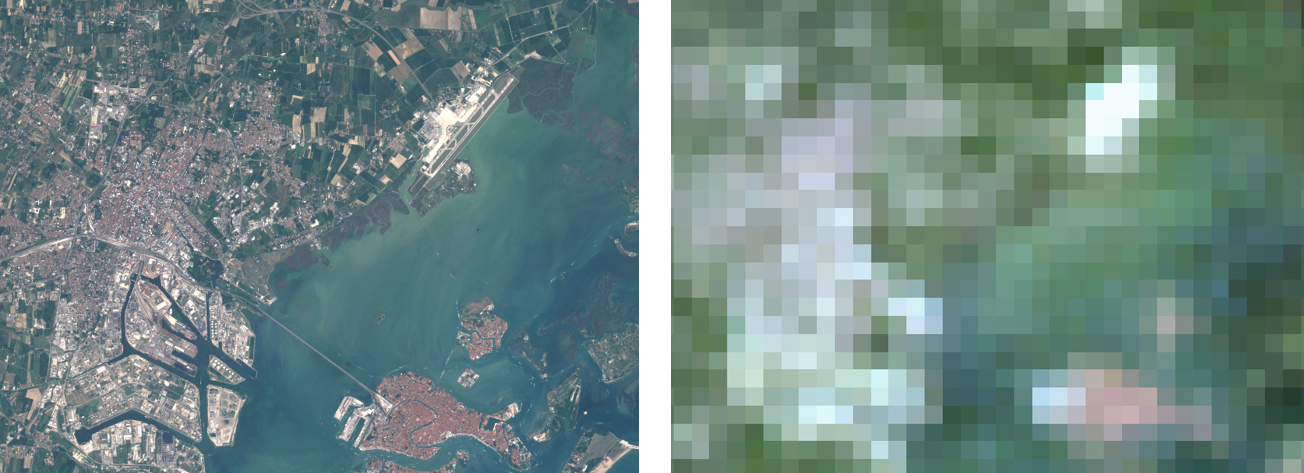
\includegraphics[width=0.75\textwidth]{SentinelVsModis.png}
  \caption{Comparaison d'une image Sentinel 2 (à g.) avec une image MODIS (à d.), en RGB}
  \label{fig:ml}
\end{figure}

Les résolutions de ces images satellites sont donc grandement meilleures que celles acquises par satellites MODIS. Leur mise à disposition du public étant elle aussi gratuite, on comprend leur intérêt. 
Néanmoins, la mission de l'Esa est récente : peu de données sont actuellement disponibles. La courverture temporelle, c'est-à-dire la fréquence à laquelle le satellite passe au-dessus d'une même zone, est également assez faible. Un seul des deux satellites ayant été lancé, le renouvellement des données se fait de manière hebdomadaire, alors que les satellites MODIS renouvellent les données deux fois par jour. 

\subsection{Classification et Machine Learning}

Pour exploiter ces données, il est nécessaire de les classifier. On cherche en effet à distinguer les différentes caractéristiques des sols observés. Les données multispectrales à traiter représentant une quantité très importante, leur classification se fait à travers des algorithmes de "Machine Learning", défini en ces termes : 

\textit{L'apprentissage automatique (Machine Learning en anglais), champ d'étude de l'intelligence artificielle, concerne la conception, l'analyse, le développement et l'implémentation de méthodes permettant à une machine (au sens large) d'évoluer par un processus systématique, et ainsi de remplir des tâches difficiles ou impossibles à remplir par des moyens algorithmiques plus classiques.\footnote{\href{https://fr.wikipedia.org/wiki/Apprentissage_automatique}{Apprentissage automatique}}}

\paragraph{}
Le machine learning se sépare en trois type d'apprentissage :
\begin{itemize}
  \item[>] L'apprentissage non-supervisé, qui consiste à donner à notre algorithme uniquement les données à classifier et à le laisser établir les différentes classes à partir des ensembles qui se séparent le mieux.
  \item[>] La régression, qui cherche à définir les données à l'aide d'une loi mathématique.
  \item[>] L'apprentissage supervisé, pour lequel il faut définir, en plus des données à traiter, des ensembles de vecteurs représentatifs de chacune des classes et déjà classés. Les vecteurs classés manuellement vont servir d’entraînement pour l'apprentissage et donc pour trouver les frontières qui séparent le mieux nos différentes classes.
\end{itemize}

\paragraph{}
Dans le cas de la surveillance d'occupation des sols, on utilise souvent des méthodes supervisées, car il est relativement aisé de reconnaître à l'œil les différents types de zones au sol (eau, champs, villes, ...). Là encore, il existe plusieurs familles d'algorithmes d'apprentissage supervisé, on différenciera dans un premier temps les algorithmes linéaires et non-linéaires. Dans la famille des algorithmes non-linéaire, on trouve des algorithmes intrinsèquement multi-classes (tel que l'algorithme dit des k-plus proches voisins que nous détaillerons plus tard), et les algorithmes binaires.
\label{DiagAlg}
\begin{center}
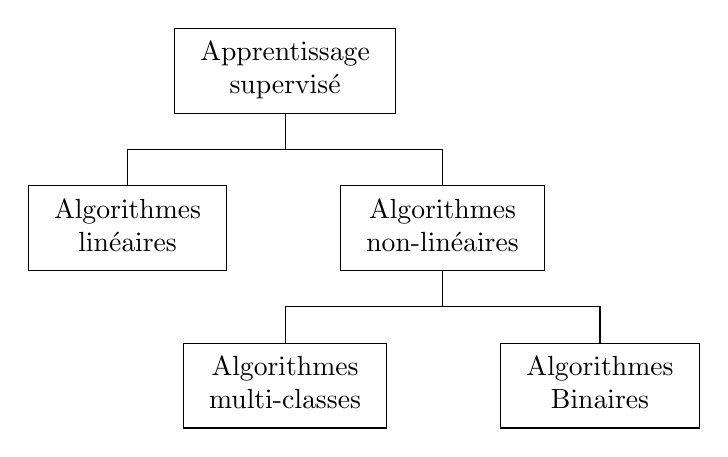
\begin{tikzpicture}
\begin{scope}
\node (AS) at (0,4.9) [rectangle,draw] {\begin{tabular}{c}Apprentissage\\ supervisé\end{tabular} };
\node (ASL) at (-2,2.9) [rectangle,draw] {\begin{tabular}{c}Algorithmes\\ linéaires\end{tabular} };
\node (ASNL) at (2,2.9) [rectangle,draw] {\begin{tabular}{c}Algorithmes\\ non-linéaires\end{tabular} };
\node (ASIM) at (0,0.9) [rectangle,draw] {\begin{tabular}{c}Algorithmes\\ multi-classes\end{tabular} };
\node (ASNM) at (4,0.9) [rectangle,draw] {\begin{tabular}{c}Algorithmes\\Binaires\end{tabular} };
\draw (AS) -- (0,3.9);
\draw (0,3.9) -| (ASNL);
\draw (0,3.9) -| (ASL);
\draw (ASNL) -- (2,1.9);
\draw (2,1.9) -| (ASIM);
\draw (2,1.9) -| (ASNM);
\end{scope}
\end{tikzpicture}
\captionof{figure}{Diagramme des différents algorithme de classification.}
\end{center}
%pas sûr que le diagramme soit utile finalement...
\paragraph{}
Pour les algorithmes intrinsèquement multi-classes, il suffit de stocker les vecteurs d’entraînement et d'appliquer directement la classification à l'ensemble des données, il n'y a donc pas d’entraînement à proprement parler.
\paragraph{}
Les algorithmes binaires, quant à eux, demandent un peu plus de travail. Dès que l'on veut traiter plus de deux classes, il faut faire plusieurs entraînements, en se ramenant chaque fois à un problème binaire. Là encore, il y a deux approches possibles en fonction des algorithmes :
 \begin{itemize}
   \item[>] La première approche s'appelle "un contre tous", elle consiste ,comme son nom l'indique, à prendre chaque classe et à l'opposer à l'ensemble des autres classes. On obtient alors n problèmes binaires et pour un élément à classifier, en cas d'ambiguïté, la classe qui obtient le plus de "votes" favorables est choisie.
   \item[>] La seconde méthode est le "un contre un", toutes les classes sont "opposées" successivement, deux à deux, et de la même façon c'est la classe qui obtient le plus de "votes" favorables qui est choisie. La principale différence réside dans le fait qu'il y ait dans ce cas ${n \choose 2}=\frac{n(n-1)}{2}$ entraînements à réaliser.
 \end{itemize}

\paragraph{L'évaluation\newline}
Pour évaluer la qualité des résultats donnés par ces algorithmes, on procède à une phase d'entraînement suivie d'une phase de test. 
On utilise pour cela un ensemble dont on connaît les classes. On va alors diviser cet ensemble en deux sous-ensembles. Le premier sous-ensemble contiendra à la fois les caractéristiques des points et leurs classes respectives. Il servira à entraîner l'algorithme. Celui-ci va ainsi apprendre quelles sont les caractéristiques de chaque classe. Le deuxième sous-ensemble contiendra uniquement les caractéristiques des points. On pourra ensuite comparer les classes inférées par l'algorithme aux classes attendues. On pourra alors quantifier la qualité des résultats à l'aide de la matrice de confusion correspondante. 

\begin{figure}[H]
  \centering
    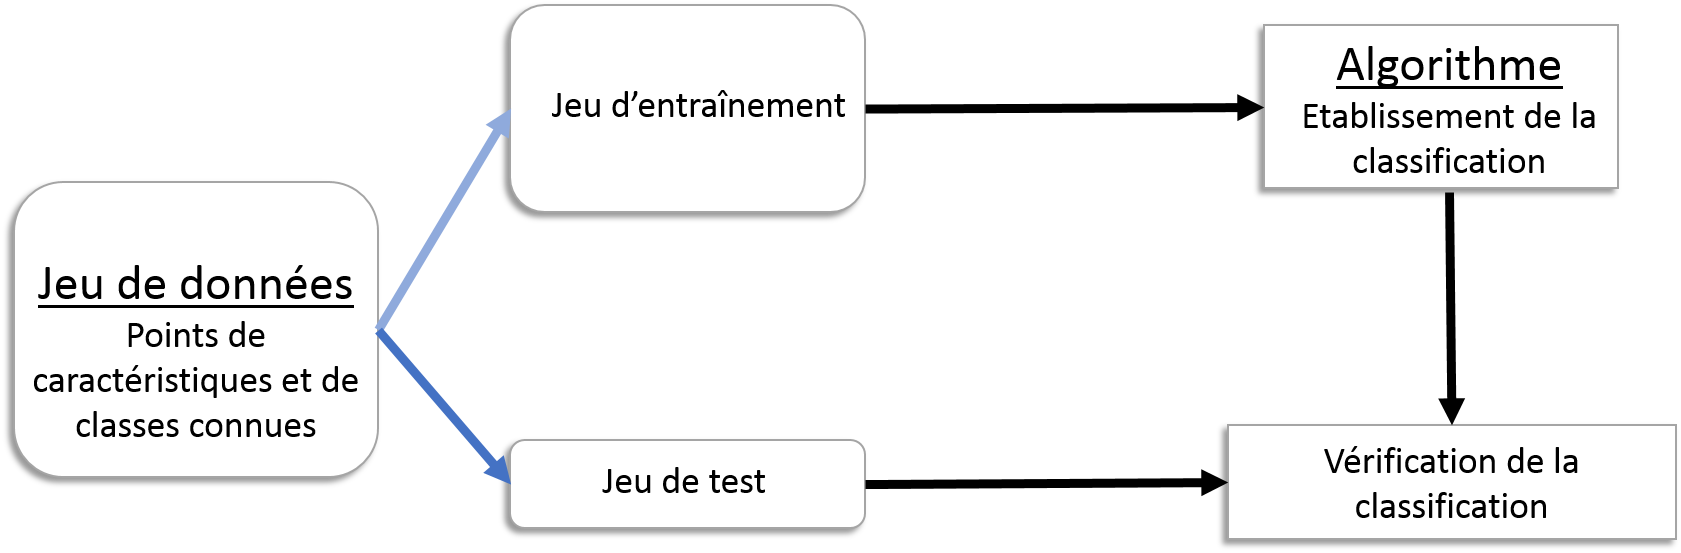
\includegraphics[width=0.75\textwidth]{mlProcess.png}
  \caption{Machine Learning}
  \label{fig:ml}
\end{figure}

\subparagraph{La matrice de confusion\newline}
La matrice de confusion est le principal outil de mesure de la qualité d'une classification. Elle compare en effet la classification prédite par l'algorithme (en lignes) à la classification réelle (en colonnes). \ref{ConfMat}
La diagonale représente le nombre d'éléments bien classés. 
Plusieurs critères sont issus de cette matrice, sous forme de pourcentage. Deux critères sont donnés par classe : la précision (precision) et le rappel (recall). La précision est la quantité d'éléments bien classés, sur le nombre d'éléments réels de cette classe. Le rappel est la quantité d'éléments bien classés, sur le nombre d'éléments prédits par l'algorithme dans cette classe.
Un autre critère est donné de manière global : l'exactitude (accuracy en anglais), qui est la trace de la matrice sur le nombre total d'éléments. Autrement dit, l'exactitude est le pourcentage de données bien classées. C'est principalement ce critère qu'on retiendra.

\begin{figure*}
\caption{Matrice de confusion pour un exemple à trois classes.}
\label{ConfMat}
\begin{center}
\renewcommand{\arraystretch}{3}
\begin{tabular}{|c|c|c|c|c|c|}
\hline
 \multicolumn{2}{|c|}{\multirow{2}{*}{}} & \multicolumn{3}{|c}{Classes Prédites} &  \\
 \cline{3-6}
  \multicolumn{2}{|c|}{} & Classe 1 & Classe 2 & Classe 3 & Précision\\
  \hline
 \multirow{3}{*}{\begin{turn}{90} Classes Théoriques\end{turn}} & Classe 1 & $N_{11}$ & $N_{12}$ & $N_{13}$ & $\frac{N_{11}}{N_{11} + N_{12} + N_{13} }$\\
 \cline{2-6}
  & Classe 2 & $N_{21}$ & $N_{22}$ & $N_{23}$ & $\frac{N_{22}}{N_{21} + N_{22} + N_{23} }$\\
  \cline{2-6}
  & Classe 3 & $N_{31}$ & $N_{32}$ & $N_{33}$ & $\frac{N_{33}}{N_{31} + N_{32} + N_{33} }$\\
  \cline{2-6}
  & Recall  & $\frac{N_{11}}{N_{11} + N_{21} + N_{31} }$ & $\frac{N_{22}}{N_{12} + N_{22} + N_{32} }$ & $\frac{N_{33}}{N_{13} + N_{23} + N_{33} }$ & $\frac{N_{11} + N_{22} + N_{33}}{Nb echantillons}$\footnote {ce résultat donne la fidélité de la classification par rapport à l'image initiale} \\
\hline
\end{tabular}
\end{center}
\end{figure*}



\subsection{Motivation du projet et cahier des charges}

Les données Sentinel 2 étant très récentes, nous faisons partie des premiers à les analyser et aucun article à leur sujet n'a encore été publié. Leur analyse et leur classification relève donc de la recherche. 
Bien que ce projet s'étende sur une durée assez courte (6 semaines), les objectifs fixés étaient :
\begin{itemize}
  \item[>] Définir les principaux intérêts des images multispectrales Sentinel 2.
  \item[>] Etablir une classification de la surface terrestre (suivi d'occupation des sols) en trois classes ("Eau", "Urbain","Champ") à partir d'une image de la base de données Sentinel 2.
  \item[>] Tester les algorithmes de Machine Learning les plus répandus.
\end{itemize}

  Dans un but de répétabilité, nous avons testé et optimisé toutes nos méthodes de machine learning sur une unique image hyperspectrale (dont une vue en RGB est donnée en figure \ref{fig:veniseRGB}).
 


\section{Etat de l'Art}
\subsection{Travaux scientifiques}
%parler des articles qu'Aurélien a trouvé pour la soutenance

Les données multispectrales des satellites MODIS sont largement utilisées par la communauté scientifique. Ici on présentera trois publications qui utilisent différentes approches de la surveillance satellite.

\paragraph{}
L'analyse des données multispectrales peut se faire en calculant des indices particuliers, comme le NDVI (normalized difference vegetation index). Le NDVI permet d'établir la présence ou l'absence de végétation dans une zone. En effet, les plantes chlorophylliennes absorbent fortement la lumière rouge et réfléchissent la lumière proche infrarouge : la différence normalisée d'intensité entre ces deux bandes correspond à l'indice NDVI. 
\begin{equation}
NDVI=\frac{NIR-VIS}{NIR+VIS}
\end{equation}
Où NIR correspond à l'intensité lumineuse dans le proche infrarouge et VIS dans le rouge.\newline
Une valeur proche de 1 indique la présence de végétation, et une valeur proche de 0 son absence. L'utilisation de cet indice est très courante. Il a ainsi été utilisé pour l'étude de la désertification de zones dues à l'activité humaine\cite{desert} par Meng-Lung et al.

\begin{figure}[H]
  \centering
    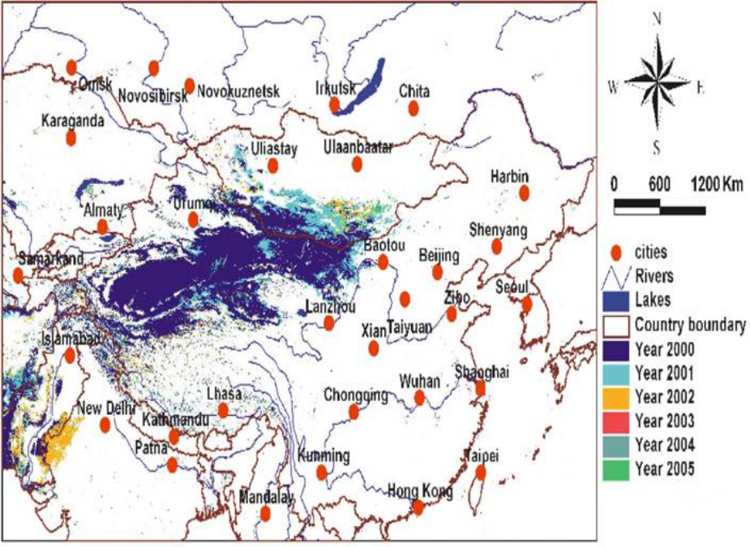
\includegraphics[width=0.5\textwidth]{etudeDesertification.png}
  \caption{Etude de la désertification, image tirée de l'article \textit{Fuzzy model based assessment and monitoring of desertification using MODIS satellite imagery}, Meng-Lung Lin et al. (2009)}
  \label{fig:etudeDesert}
\end{figure}

\paragraph{}
En outre, les données satellites peuvent servir à analyser la qualité de l'air au niveau du sol et, entre autres, en déduire la présence d'évènements exceptionnels comme des feux de forêt ou du brouillard\cite{airSurv}. 

\begin{figure}[H]
  \centering
    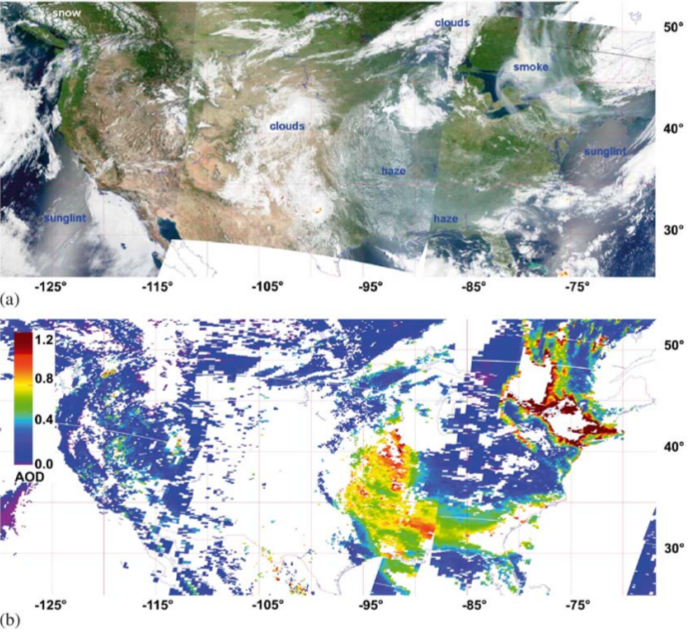
\includegraphics[width=0.5\textwidth]{surveillanceAtmo.png}
  \caption{Suivi atmosphérique, image tirée de l'article \textit{Qualitative and quantitative evaluation of MODIS satellite sensor data for regional and urban scale air quality}, Engel-Cox et al. (2004)}
  \label{fig:survAtmo}
\end{figure}

\paragraph{}
Plus proche de notre projet, la classification peut se faire par des algorithmes de machine learning. Cette approche a été suivie dans l'étude menée par M.A. Friedl et al. 

\begin{figure}[H]
  \centering
    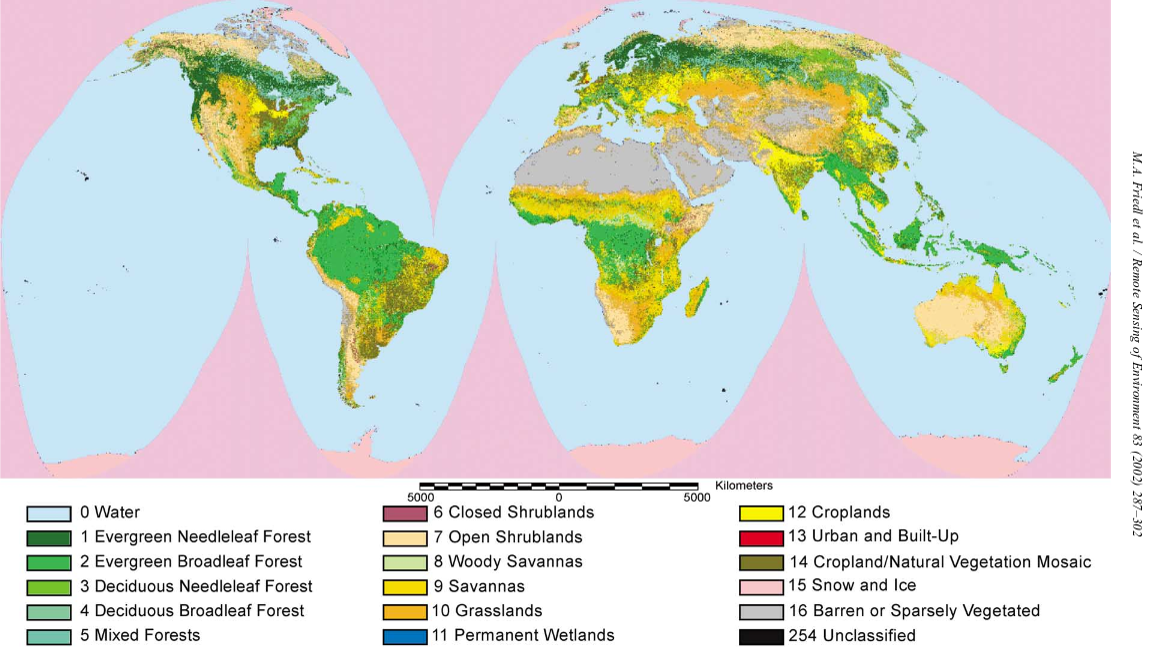
\includegraphics[width=0.75\textwidth]{classifSols.png}
  \caption{Classification des sols, image tirée de l'article \textit{Global land cover mapping from MODIS: algorithms and early results}, M.A. Friedl et al. (2002)}
  \label{fig:clSols}
\end{figure}

\subsection{Les logiciels de classification}
Nous allons ici présenter quelques logiciels qui permettent de faire de la surveillance d'occupation des sols. Il en existe un très grand nombre, c'est pourquoi nous nous sommes concentrés sur les principaux logiciels utilisés dans le domaine.
\paragraph{QGIS}
\paragraph{}
QGIS est un logiciel libre multiplateforme, qui permet de traiter les formats usuels d'image satellite, mais aussi d'y ajouter des couches vectorielles pour délimiter des polygones ou classifier des zones géographiques.
De plus, la communauté de QGIS a développé de nombreux "plugins" (modules d'extension) permettant d'appliquer différents algorithmes de machine learning.\newline
Le logiciel SAGA, intégré à QGIS, utilise l'algorithme de ressemblance maximale, qui permet de faire une classification statistique des pixels. Ayant choisi des polygones d'entraînement, ils vont être assimilés à des lois normales et à partir de leurs moyennes et de leurs variances, les pixel inconnus vont appartenir à la classe à laquelle ils ont le plus de chance d'appartenir.
Semi-Automatic Classification Plugin, permet également d'obtenir des classifications à partir d'image à l'aide de différents algorithmes.
OrfeoToolBox est un autre logiciel qui a la possibilité d'être utilisé via Qgis et qui peut réaliser une classification d'images satellite.

\paragraph{ENVI}
\paragraph{}
ENVI ({\href{http://www.exelisvis.fr/ProduitsetServices/LesproduitsENVI/ENVI.aspx}{ENvironment for Visualizing Images}}) est un logiciel propriétaire, payant, sous licence commerciale. Il permet de traiter efficacement les données satellites à l'aide de plusieurs algorithmes dont celui de la ressemblance maximum. C'est un logiciel très utilisé dans l'industrie et qui est relativement facile d'utilisation.
\paragraph{ArcGIS}
\paragraph{}
Parmi les logiciels payant sous licence propriétaire, on peut aussi noter ArcGIS, développé par la société Esri (Environmental Systems Research Institute, Inc.). Il contient également une boîte à outil de traitement des images géographiques relativement complète.

\section{Méthode et organisation}
\subsection{Processus}
\paragraph{}
L'objectif de ce projet était de classifier une zone géographique à partir des images satellites fournies par Sentinel-2. Par souci de lisibilité, nous avons choisi de présenter les résultats sous la forme d'images RGB composées d'autant de teintes qu'on a choisi de classes (par exemple pour une classification tri-classes, l'image finale a trois teintes : rouge, verte et bleue).
\paragraph{}
Afin d'arriver à ce résultat, il a fallu traiter les données fournies par l'ESA. Celles-là ont donc subi un processus résumé ci-dessous et expliqué après : \\\\
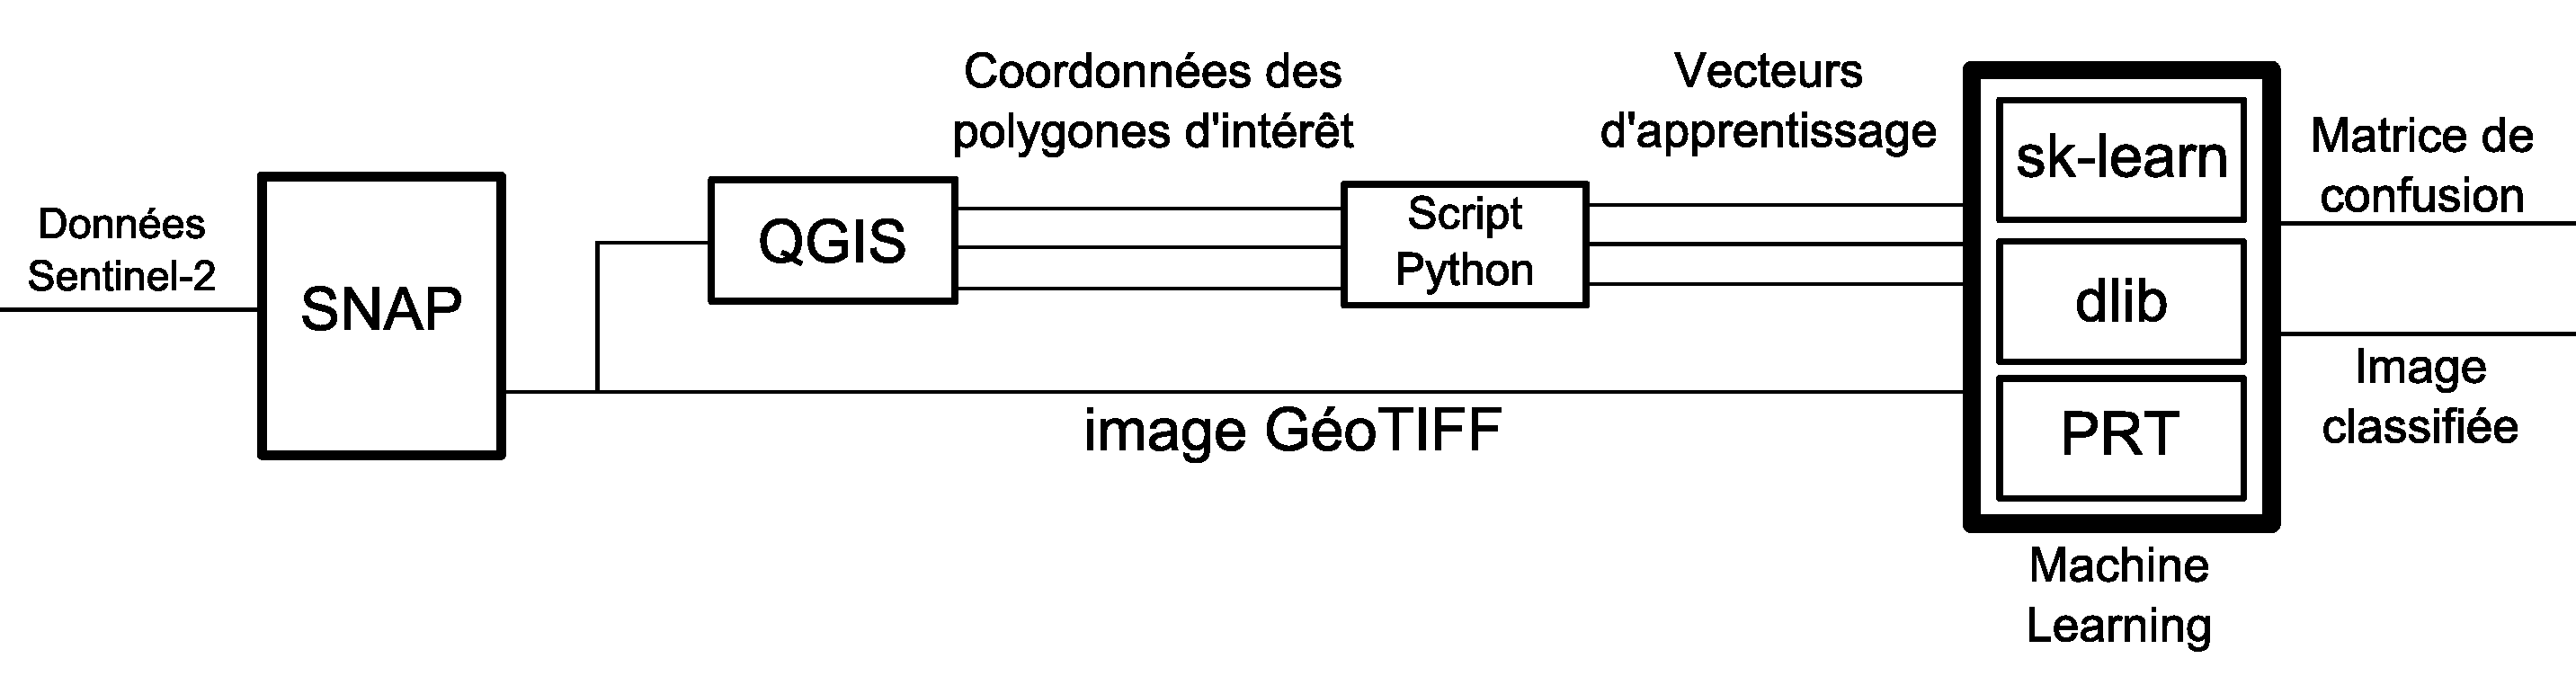
\includegraphics[scale=0.3]{process_Multispec.pdf}
\subsubsection{SNAP}
\paragraph{}
SNAP\footnote{\href{http://step.esa.int/main/toolboxes/snap/}{SNAP | STEP}} (ou Sentinel Application Platform) est un logiciel open-source et gratuit développé par l'Agence Spatiale Européenne (ESA). Il est le seul capable d'ouvrir les données de Sentinel-2 et d'afficher les différentes bandes de l'image multispectrale. Pour pouvoir manipuler simplement l'image (l'originale étant très volumineuse et dans un format complexe et inadapté), nous avons donc sélectionné une sous-image que nous avons exportée au format GéoTIFF.
\subsubsection{QGIS}
\paragraph{}
QGIS\footnote{\href{http://www.qgis.org}{Site Officiel de QGIS}} est un logiciel de cartographie libre publié sous licence GPL. Afin de pouvoir utiliser les algorithmes d'apprentissage automatique, nous avons besoin de sélectionner des pixels dont on connaît par avance la classe (urbain, champ ou eau). Sous QGIS, nous avons donc tracé des polygones autour de zones ne contenant qu'un seul type de classe : des polygones autour d'une région ne contenant que de l'eau, puis que des champs, puis que de la ville. Nous avons ensuite exporté les coordonnées de ces polygones.
\subsubsection{Script Python}
\paragraph{}
Comme il a été précédemment écrit, pour pouvoir utiliser les algorithmes d'apprentissage automatique, il faut choisir sur l'image des pixels dont on connaît par avance la classe. Nous avons donc écrit un script sous Python en utilisant l'image sélectionnée et les coordonnées des polygones sélectionnés auparavant. Nous avons extrait les valeurs des 13 bandes de tous les pixels contenus à l'intérieur des polygones. Ces "pixels" de 13 bandes formeront les vecteurs d'entraînement de nos algorithmes d'apprentissage automatique. On enregistre alors trois listes de pixels sous format texte : une liste des pixels "urbain", une autre contenant les pixels "champs" et enfin une dernière liste avec les pixels "eau".
\subsubsection{Sk-learn, dlib et PRT}
\paragraph{}
Sk-learn\footnote{\href{http://scikit-learn.org}{scikit-learn.org}}, dlib\footnote{\href{http://dlib.net}{dlib.net}} et PRT\footnote{\href{https://github.com/covartech/PRT}{github.com/covartech/PRT}} sont trois bibliothèques permettant d'utiliser des algorithmes d'apprentissage automatique. Elles sont respectivement publiées sous Licence BSD, Licence Logicielle Boost et Licence MIT, toutes trois des licences de logiciel libre. Toutes les trois sont écrites dans un langage différent, respectivement Python, C++ et MatLab. L'idée était de tester les différentes implémentations, de comparer leur rapidité et leur facilité d'utilisation. Nous avons utilisé quatre algorithmes classiques pour la classification : la méthode aux moindres carrés, celle des K-Nearest Neighbors, l'Analyse Discriminante Linéaire et des Machines à Vecteur de Support. Les résultats seront exposés et comparés plus loin dans le rapport. Nous avons donc utilisé différents algorithmes sous différentes implémentations sur notre image. Finalement, nous avons créé une image RGB avec en rouge les zones urbaines, en vert les zones agricoles et en bleu l'eau. Associé à cette image, nous avons aussi calculé une matrice de confusion, outil mathématique permettant d'évaluer rapidement et finement la qualité de la classification opérée par un des algorithmes d'apprentissage automatique.
\subsection{Organisation du projet}
\subsubsection{Répartition du travail}
\paragraph{}
Dans un premier temps, il a fallu tous nous familiariser avec les notions d'apprentissage automatique et avec les différents logiciels à utiliser. Nous avons donc tous les quatre travaillé en commun. Chacun a donc appris à utiliser SNAP, puis QGIS. Quand nous avons commencé à mieux comprendre le projet et à être plus à l'aise, nous nous sommes partagés les tâches.
\paragraph{}
Pendant que Youna, Aurélien et Pierre continuaient de se documenter sur l'apprentissage automatique, Benjamin travaillait sur le script Python permettant l'extraction des pixels "intéressants". C'est donc Benjamin qui a codé ce bloc. Une fois cette partie terminée, à l'aide des pixels extraits, nous avons tous pu commencer à implémenter les algorithmes d'apprentissage automatique. Chacun a choisi un langage différent : Benjamin a choisi le C++, Aurélien le Python, Youna et Pierre le langage MatLab. Nous avons tous codé de a à z la méthode des moindres carrés car celle-ci est la méthode la plus simple et qu'elle permet de comprendre tout le principe de la classification. Cette première méthode a donc eu un intérêt pédagogique.
\paragraph{}
C'est à partir de ce moment que nous avons commencé à paralléliser les tâches : chacun a implémenté les algorithmes d'apprentissage automatique avec différents langages et différentes bibliothèques : Benjamin a utilisé dlib sous C++, Aurélien sk-learn sous Python, Youna ANN (Approximate Nearest Neighbors, publiée sous Licence LGPL) sous C++ pour coder la méthode des k plus proches voisins et Pierre a utilisé PRT sous MatLab.
\subsubsection{Mise en commun du travail}
\paragraph{}
Afin d'organiser au mieux le code que nous avons écrit, nous avons utilisé Git. Cela nous a permis de partager nos différents codes ainsi que nos différents résultats. Par ailleurs, nous avons choisi d'écrire notre rapport sous LaTeX. Git s'est donc aussi révélé très utile quand il s'est agi de mettre en commun les contributions de chacun dans la rédaction. À ce propos, nous avons décidé de nommer un coordinateur pour la rédaction du rapport : Pierre et un autre coordinateur pour la soutenance : Youna.
\subsubsection{Rencontres avec le tuteur}
\paragraph{}
Le projet s'est intégralement structuré autour de réunions hebdomadaires avec notre tuteur Nicolas Brodu. Ces réunions avaient à la fois pour but de rapporter les progrès que nous avions faits mais aussi de nous apprendre les bases de Machine Learning. Ces réunions ont donc été capitales dont la compréhension du sujet et donc dans l'avancement du projet. Le projet ayant duré 6 semaines, nous avons fait 6 réunions. Voici donc l'historique des réunions et les points abordés.
\paragraph{04/11 :} Dans un premier temps, Nicolas Brodu nous a exposé ce sur quoi il travaillait, il a aussi dressé un court état de l'art de la classification des sols. Il nous a ensuite proposé plusieurs sujets portant sur ce domaine et nous avons alors choisi de développer l'aspect Apprentissage Automatique avec pour objet les images multispectrales de Sentinel-2. Une fois ce choix fait, nous avons établi avec lui un cahier des charges.
\paragraph{10/11 :} L'enjeu de la première semaine était de se familiariser avec les images multispectrales, d'apprendre à se servir de SNAP (ouvrir une image, extraire une sous-image et l'exporter au bon format) de QGIS (ouvrir la sous image, tracer et extraire des polygones autour de zones d'intérêt). C'est aussi au cours de cette semaine que nous avons commencé à coder le script Python pour extraire les valeurs des pixels contenus dans les zones d'intérêt. Nous avons donc rapporté à notre tuteur notre avancement et nos difficultés quant à l'écriture du script. M. Brodu a également profité de cette réunion pour nous apprendre les principes de l'apprentissage automatique et plus particulièrement du  Machine Learning  linéaire (notamment la classification aux moindres carrés).
\paragraph{18/11 :} C'est à partir de cette réunion que nous avons pu montrer les premiers résultats de classification à notre tuteur. Nous avons également pu montrer que la bande 10 était inutilisable sur l'image que nous avions prise pour travailler et que les 12 autres bandes étaient nécessaires (en enlevant une ou plusieurs bandes la précision se dégradait rapidement à l'œil nu). M. Brodu nous alors introduit la matrice de confusion, outil permettant d'évaluer quantitativement la justesse de classification. Il a également exposé d'autres algorithmes d'apprentissage automatique : la LDA\footnote{\href{https://en.wikipedia.org/wiki/Linear_discriminant_analysis}{Linear Discriminant Analysis}} (Analyse discriminante linéaire) et la PCA\footnote{\href{https://en.wikipedia.org/wiki/Principal_component_analysis}{Principal Component Analysis}} (Analyse en Composantes Principales). Face au temps qu'il nous restait, il était exclu d'implémenter nous même chaque algorithme d'apprentissage automatique. C'est pourquoi nous avons utilisé des bibliothèques contenant déjà les algorithmes. Notre tuteur nous a suggéré plusieurs bibliothèques, toutes sous licences libres. À propos de MatLab, c'est effectivement un logiciel payant et non libre. Nous avons malgré tout continué à l'utiliser en sachant que s'il fallait passer à une alternative libre, nous pourrions toujours utiliser Octave\footnote{\href{https://www.gnu.org/software/octave/}{GNU Octave}}, qui a l'avantage d'avoir presque la même syntaxe que MatLab.
\paragraph{25/11 :} Nous avons eu peu de nouveaux résultats à rapporter cette semaine : nous nous sommes concentrés sur l'apprentissage des méthodes des différentes bibliothèques. Nous avons quand même pu confirmer grâce à l'utilisation de la matrice de confusion que la méthode des moindres carrés fonctionnait surprenamment bien pour une méthode aussi simpliste. Si la méthode la plus basique de classification fonctionne aussi bien, quelle précision pouvons nous espérer avec des méthodes plus complexes ? Nous avons voulu apporter une réponse à cette question et c'est pourquoi M. Brodu nous a expliqué les principe du Machine Learning non linéaire en commençant par développer deux méthodes : les SVM\footnote{\href{https://en.wikipedia.org/wiki/Support_vector_machine}{Support Vector Machine}} (Machines à Vecteurs de Support) et la méthode des KNN\footnote{\href{https://en.wikipedia.org/wiki/K-nearest_neighbors_algorithm}{K-Nearest Neighbors}} (K plus Proches Voisins). Ces algorithmes ont la particularité de contenir des méta-paramètres (par exemple K pour les KNN), qu'il faut bien choisir. Notre tuteur nous a donc donné la méthode classique pour les choisir : faire de la validation croisée.
\paragraph{09/12 :} Cette réunion a été la dernière où nous avons pu exposer nos résultats. Nous avons exposé tout ce que nous avions fait et le reste de la réunion a porté sur les possibles ouvertures du projet : Faire du blanchiment (pour attribuer le même poids aux différentes bandes dans la classification), utiliser des algorithmes de super-résolution, utiliser les bandes radar de Sentinel-1, utiliser d'autres indicateurs. M. Brodu a ainsi évoqué la Malédiction de la dimensionalité (utiliser toujours plus d'indicateurs peut dégrader des résultats si l'on ne fait pas attention).
\paragraph{16/12 :}Cette dernière réunion a constitué en une soutenance blanche, nous avons fait une première présentation à notre tuteur et celui-ci nous a aidé à l'améliorer et à mieux expliquer l'apprentissage automatique à des personnes ne connaissant pas ce domaine.

\section{Résultats}
Le résultat d'une classification est une image RGB dont la couleur de chaque pixel représente la classe à laquelle il appartient selon l'algorithme. Par exemple, dans une image résultat, un pixel bleu correspond à un point identifié par l'algorithme comme étant de l'eau. Notre code couleur est résumé dans le tableau \ref{table:codeCouleur}.
\begin{figure}[H]
 \begin{center}
  \begin{tabular}{|c|c|}
    \hline
    Nature du terrain & couleur \\
    \hline
  Champ & Vert \\
  Ville &  Rouge \\
  Eau &  Bleu \\
  Boue & Marron \\
    \hline
  \label{table:codeCouleur}
  \end{tabular}
\caption{Code couleur des images produites par machine learning.} 
\end{center}
\end{figure}
Estimer la qualité d'un classificateur revient à estimer la qualité de l'image résultante. Pour cela, deux méthodes s'offrent à nous: la première numérique, consiste à calculer la matrice de confusion de chaque classificateur comme expliqué INSERER ICI OU CEST EXPLIQUE. Pour plus de clarté, l'exactitude sera en rouge. L'autre méthode consiste à estimer à l'œil la correspondance entre les prédictions de nos algorithmes et la réalité (les zones de référence étant elles-mêmes choisies à l'œil, ce critère n'est pas plus mauvais que l'autre). Pour immédiatement visualiser cette correspondance, nous superposons l'image de base avec l'image résultante en transparence, comme par exemple sur la figure \ref{fig:veniseLSE}.

 \subsection{Les classifications linéaires}
 
 Réaliser une classification linéaire d'un ensemble de données en différentes classes revient, en deux dimensions, à trouver la droite qui sépare au mieux deux ensembles de vecteurs. Dans la figure \ref{fig:ml_lin}, on prend l'exemple d'un ensemble de points représentant de l'eau et de l'urbain. Sur l'image, les points représentant l'eau auront une couleur plutôt bleue alors que les points représentant des zones urbaines seront plutôt rouge, voire gris. Ils sont assez bien distingués pour trouver une séparation linéaire.

\begin{figure}[H]
  \centering
    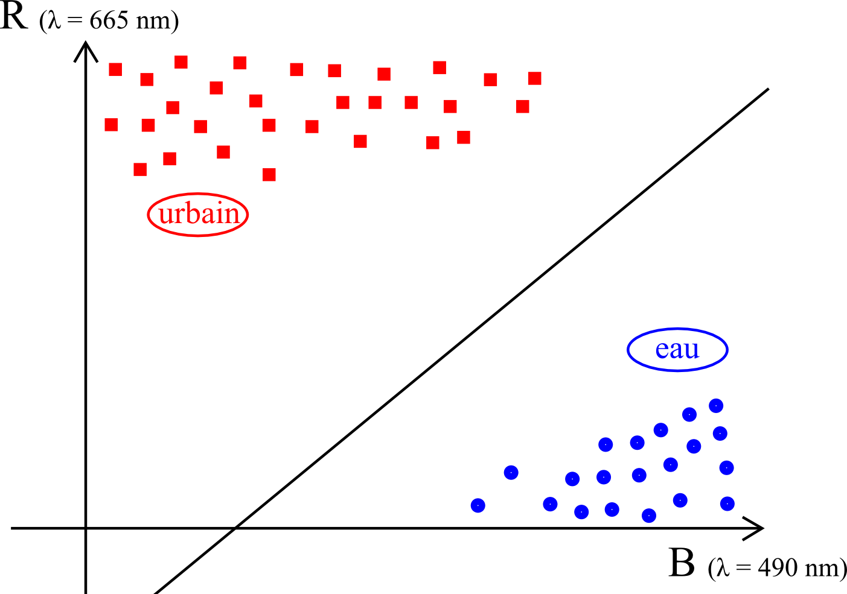
\includegraphics[width=0.5\textwidth]{ml_lin.png}
  \caption{Classification linéaire}
  \label{fig:ml_lin}
\end{figure}

Il existe plusieurs méthodes pour trouver une droite qui sépare correctement les deux ensembles de points.

\paragraph{La méthode des moindres carrés}
  La première méthode consiste à faire l'hypothèse que tous les points des deux ensembles sont alignés, et qu'on peut alors trouver une droite telle que tous les points soient à une distance de 1, pour l'une des deux classes, et de -1 pour l'autre. On se ramène alors à une optimisation linéaire qui peut être résolue par la méthode des moindres carrés.
  C'est la première classification que nous avons testée et aussi la seule que nous avons entièrement implémentée nous-mêmes. 
  
  \begin{figure}[H]
  \centering
    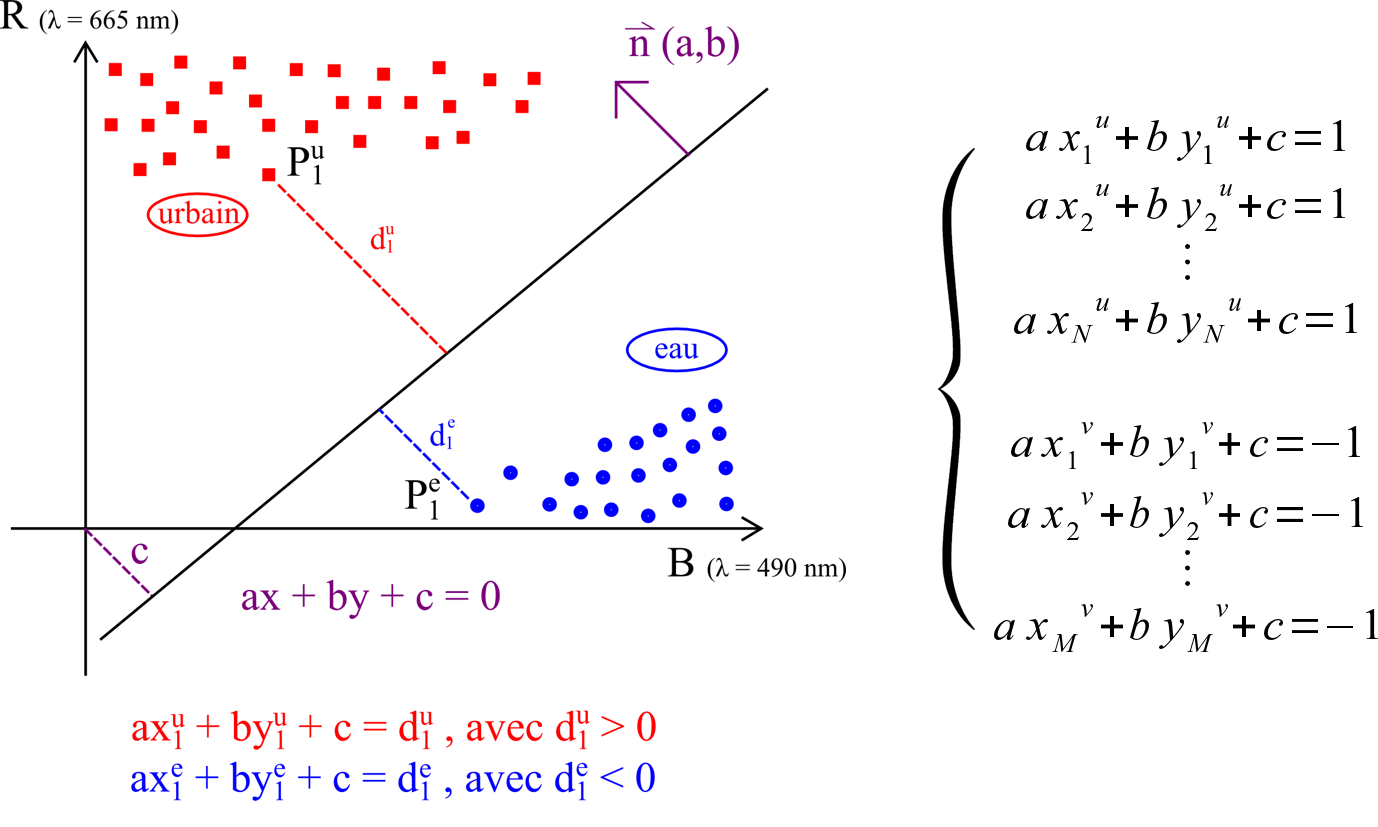
\includegraphics[width=0.75\textwidth]{ml_lse}
  \caption{Classification linéaire}
  \label{fig:ml_lse}
\end{figure}
  
\label{lineaire}
 Les résultats obtenus sont encourageants, avec une première classification qui à première vue correspond à la répartition réelle des trois classes étudiées (figure \ref{fig:veniseLSE} avec la matrice de confusion correspondante \ref{table:confLSE}).

\begin{figure}[H]
  \centering
    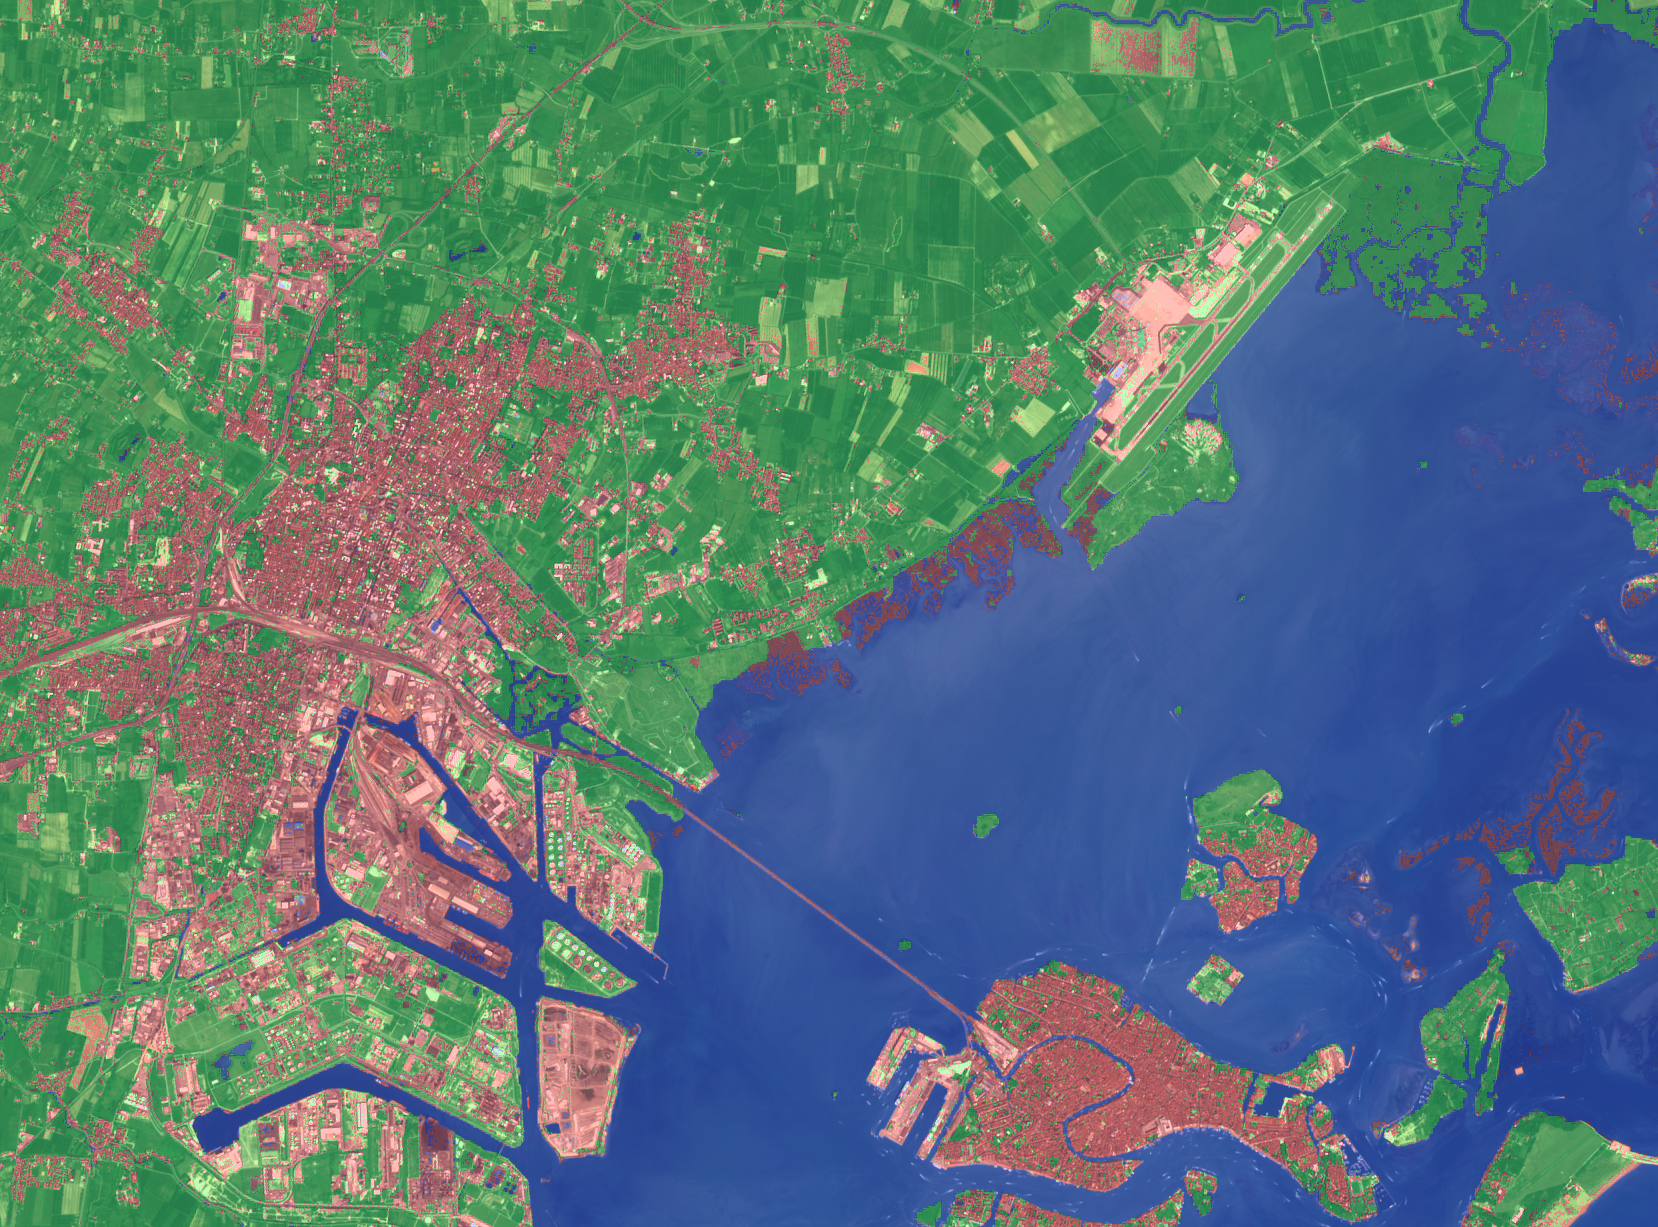
\includegraphics[width=0.75\textwidth]{veniseLSE}
  \caption{Résultat de classification avec un classificateur linéaire}
  \label{fig:veniseLSE}
\end{figure}

\begin{figure}[H]
\begin{center}
 \begin{tabular}{|c|c|c|c|c|}
  \hline
  Nature du terrain & Eau & Champ & Urbain & Rappel \\
  \hline
Eau & 10000   &   0    &   0 & 100\% \\
Champ & 0   &  9991     &   9  & 99.9\% \\
Urbain &  11   &     2712  &   7277 & 72.8\% \\
Précision & 99.9\%  & 78.9\% & 99.9\% & {\color{red}90.9\%} \\
  \hline
\end{tabular}
\end{center}
\caption{Matrice de confusion de la classification linéaire}
\label{table:confLSE}
\end{figure}

L'exactitude de cette méthode est de 90.9\%. On peut constater que l'eau est très bien classifiée, et que les erreurs proviennent majoritairement de confusions entre les champs et la ville. Il est également intéressant de voir que cette confusion n'est pas symétrique : si lez zones urbaines sont classifiées comme des champs par l'algorithme, l'inverse est beaucoup moins vrai.

\paragraph{Analyse discriminante linéaire ou de Fisher}
  Une seconde méthode consiste à utiliser l'analyse discriminante linéaire\footnote{ou analyse discriminante de Fisher}(LDA), c'est-à-dire poser l'hypothèse que chaque ensemble de points a une distribution gaussienne, et à trouver, à partir de la variance et de la moyenne de ces distributions la meilleure séparation entre les ensembles. On peut voir cette méthode comme une recherche de droite sur laquelle la projection des gaussiennes est la mieux séparé, la meilleure séparation est alors l'hyperplan perpendiculaire à cette droite. Cependant, dans la pratique, l'hypothèse de distribution gaussienne est très forte et rarement vérifiée.

\begin{figure}[H]
  \centering
    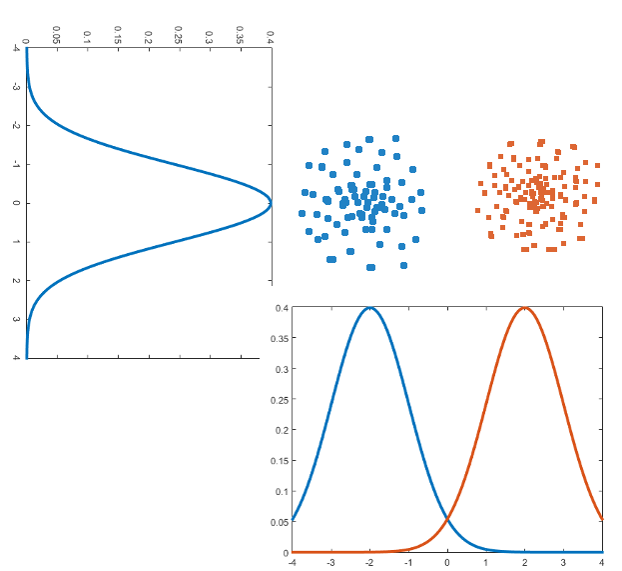
\includegraphics[width=0.4\textwidth]{ml_lda}\hfill
    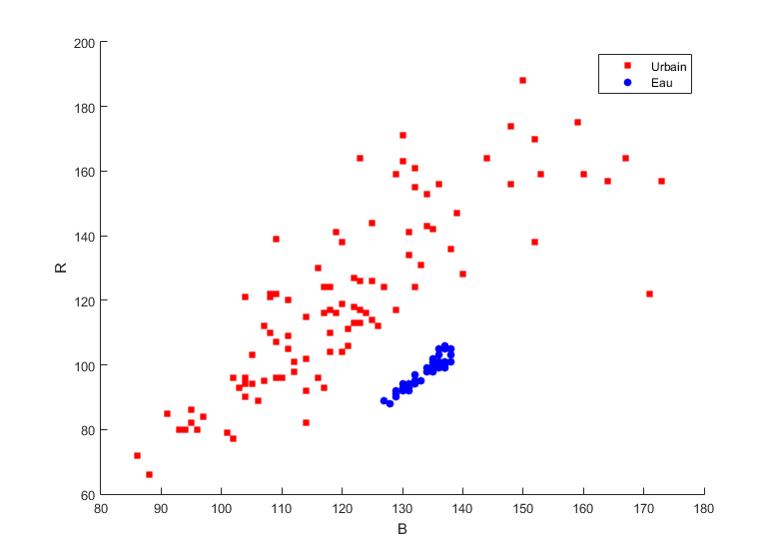
\includegraphics[width=0.5\textwidth]{ml_ldaReel}
  \caption{Analyse discriminante linéaire : hypothèse (à g.) vs repartition réelle (à d.)}
  \label{fig:ml_lda}
\end{figure}

  En effet, nous avons choisi des polygones de manière à ce qu'ils contiennent le moins de points possibles, les plus représentatifs possibles, afin de diminuer les temps de calcul. Ce faisant, nous n'avons pas pris un échantillon continu de points et l'approximation gaussienne est difficilement valable, ce qui explique les mauvais résultats obtenus, en particulier sur les zones de ville.
\begin{figure}[H]
  \centering
    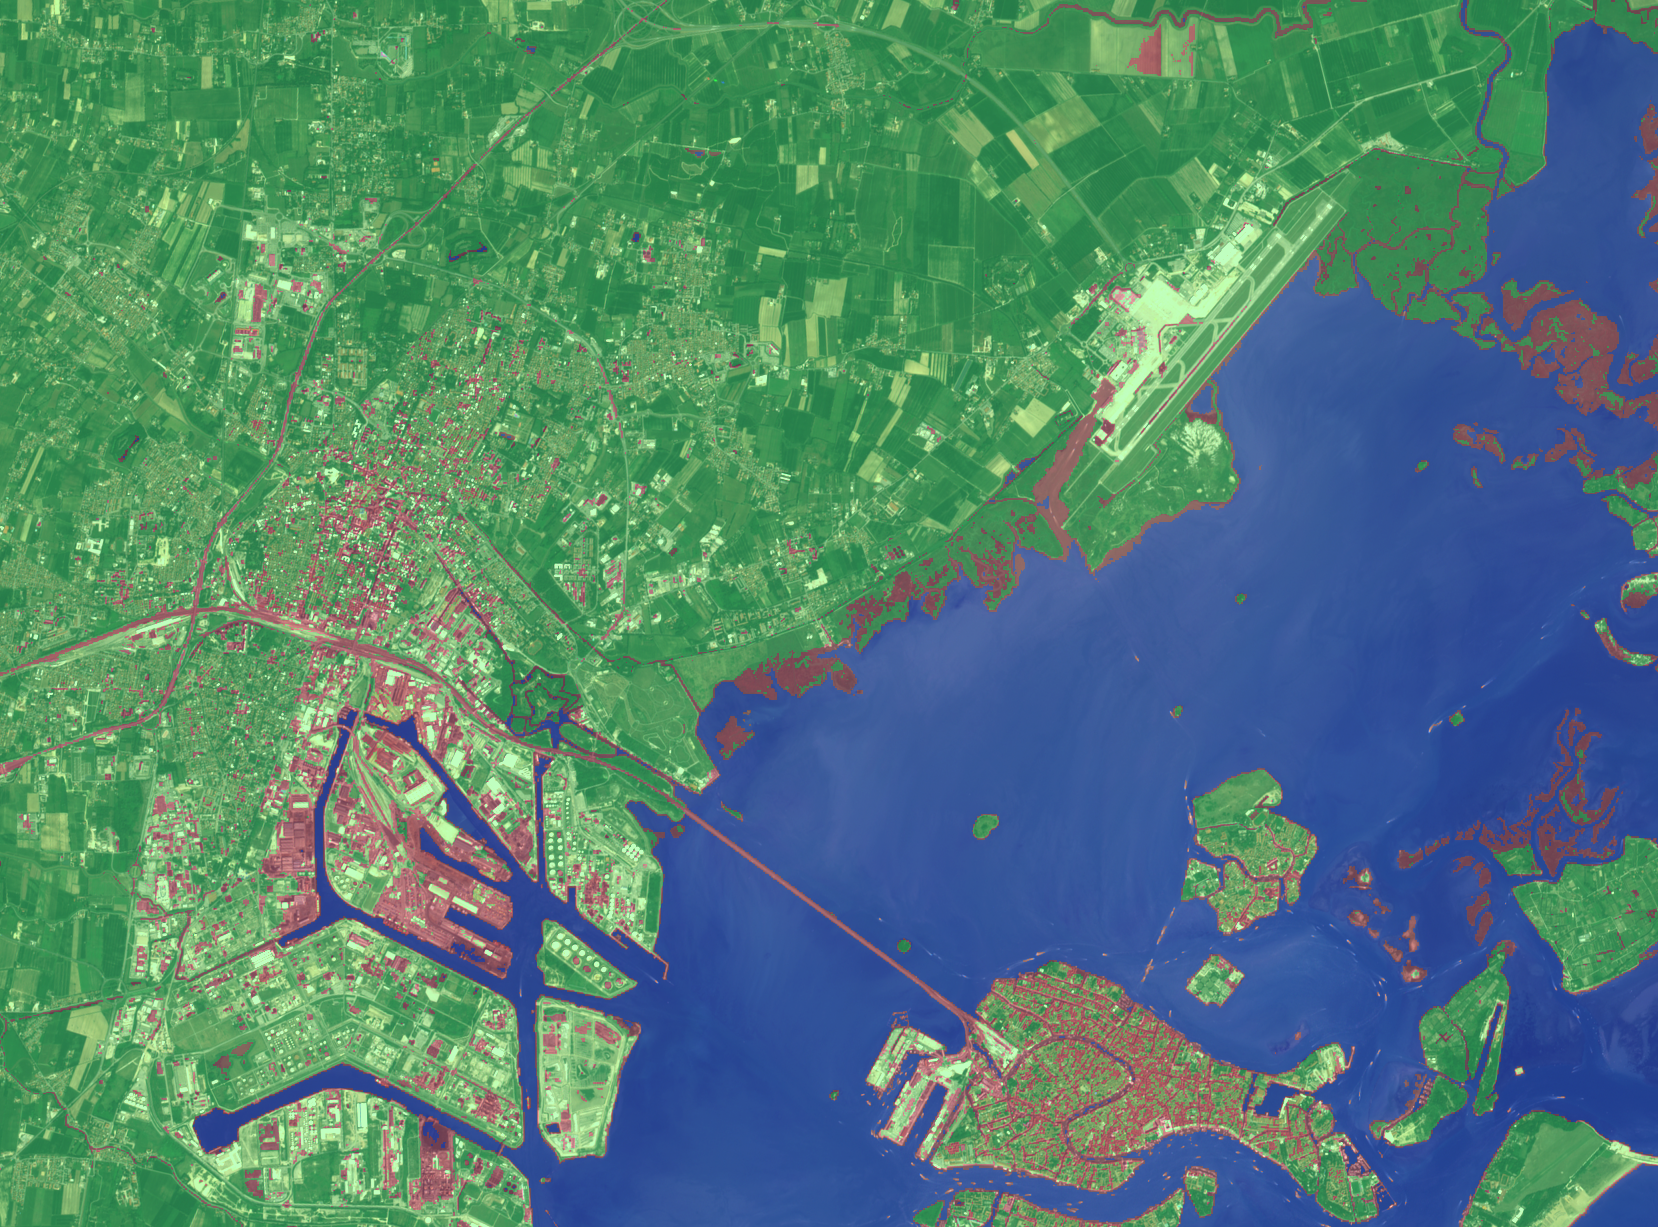
\includegraphics[width=0.75\textwidth]{venise+LDA}
  \caption{Résultat de classification avec une analyse linéaire de discriminant}
  \label{fig:veniseLDA}
\end{figure}

\begin{table}[H]
\begin{center}
 \begin{tabular}{|c|c|c|c|c|}
  \hline
  Nature du terrain & Eau & Champ & Urbain & Rappel \\
  \hline
Eau & 9966  &   0  &      34 & 99.7\% \\
Champ & 0  &  10000   &     0 & 100\% \\
Urbain &  0    &    6461  &   3539   &     35.4\% \\
Précision & 100\% & 60.7\%  &      99.0\% & {\color{red}78.4\%}\\
  \hline
\end{tabular}
\end{center}
\caption{Matrice de confusion de l'analyse avec discriminant linéaire }
\label{table:veniseLDA}
\end{table}
    
     

\subsection{Les classifications non-linéaires}

Dans certains cas, les ensembles sont impossibles à classifier de manière linéaire. Il faut alors utiliser des algorithmes non linéaires. Dans la figure \ref{fig:ml_nlin}, on souhaite classifier un ensemble de points représentant l'eau et les champs. Les points représentant l'eau sont toujours plutôt bleus, mais les points représentant les champs peuvent varier du vert au jaune, voire des teintes rouges. Les données sont alors beaucoup plus compliquées à classifier efficacement de manière linéaire. 

\begin{figure}[H]
  \centering
    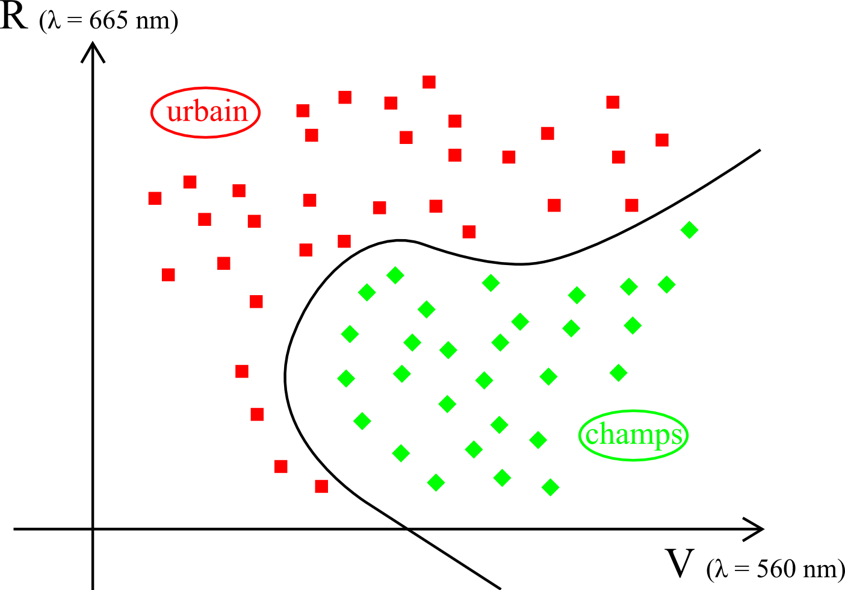
\includegraphics[width=0.5\textwidth]{ml_nlin}
  \caption{Classification non linéaire}
  \label{fig:ml_nlin}
\end{figure}

\paragraph{Machine à Vecteurs de Support (SVM) :}

Les SVM ont été développées dans les années 1990 d'après les travaux de Vladimir Vapnik. Cette approche généralise les classificateurs linéaires en cherchant une séparation linéaire de marge maximum. Pour cela, l'idée est dans un premier temps de chercher les vecteurs des différentes classes qui définissent le mieux l'enveloppe de chaque classe, et de trouver l'hyperplan qui maximise l'écart à ces vecteurs de support.

\begin{figure}[H]
  \centering
    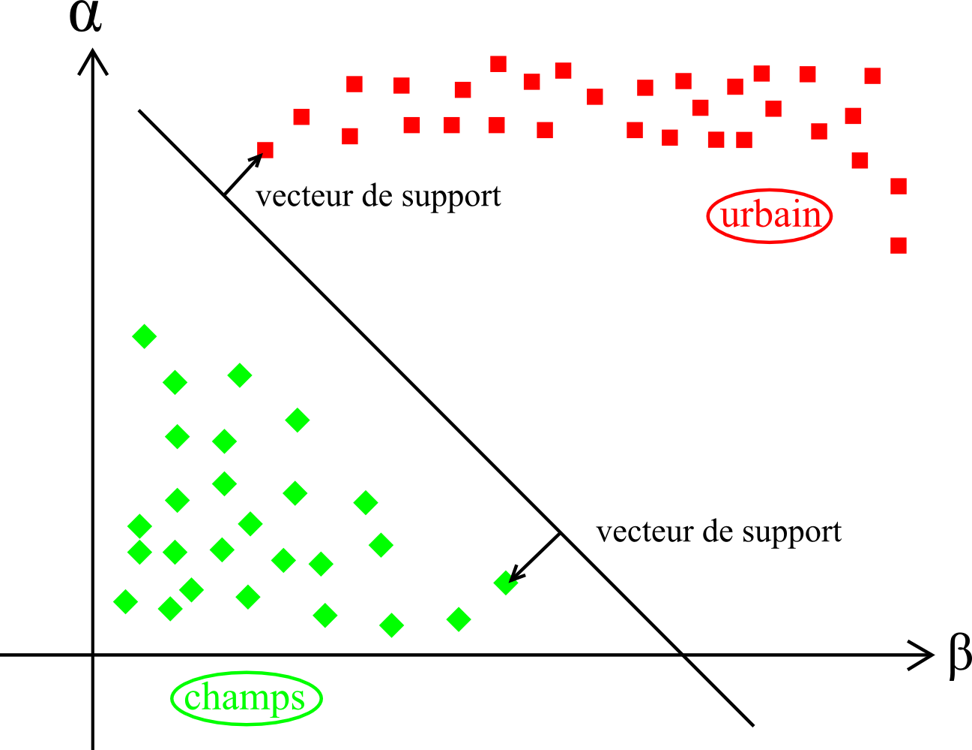
\includegraphics[width=0.5\textwidth]{ml_svm}
  \caption{Classification par SVM}
  \label{fig:ml_svm}
\end{figure}

Pour augmenter la précision de la classification, il est intéressant de trouver une frontière non-linéaire. Pour ce faire, on utilise l'astuce du noyau (ou kernel trick). Le \textit{kernel trick}\cite{aizermanSVM} consiste à remplacer le produit scalaire de l'espace considéré par l'évaluation d'une fonction (appelée noyau), on peut ramener l'étude d'un problème non séparable linéairement, à un problème linéaire. La classification admet alors des méta-paramètres, qui devront être fixés par l'utilisateur avant de réaliser l'entraînement. Afin d'optimiser l'apprentissage et la classification de notre image, il faut trouver les méta-paramètres idéaux. Pour cela, on utilise une méthode d'évaluation dite validation croisée.

\subparagraph{La validation croisée\newline}
Il s'agit d'une technique d'évaluation de la classification qui va nous permettre de maximiser la taille des polygones d'entraînement et de test. En effet, cette technique consiste à n'avoir qu'un seul jeu de polygones qui seront utilisés intégralement pour le test et pour l'entraînement. L'astuce réside ici à utiliser une partie des éléments du polygone pour l'entraînement et le reste pour le test, puis de réitérer en changeant les éléments utilisés pour le test et ainsi de suite jusqu'à ce que tous les éléments aient été utilisé pour le test.
\begin{center}
\renewcommand{\arraystretch}{4}
\begin{tabular}{c | c || c || c}
  Etape 1& Etape 2 & Etape 3\\
  \cellcolor{Periwinkle}test & \cellcolor{NavyBlue}entrainement & \cellcolor{NavyBlue}entrainement\\
  \cellcolor{NavyBlue}entrainement & \cellcolor{Periwinkle}test & \cellcolor{NavyBlue}entrainement\\
  \cellcolor{NavyBlue}entrainement & \cellcolor{NavyBlue}entrainement & \cellcolor{Periwinkle}test\\
\end{tabular}
  \captionof{figure}{Illustration de la validation croisée.}
\end{center}


Dans notre cas, on utilise deux méta-paramètres : C et $\gamma$. on sépare notre jeu de données en 5, 4 parts servant à l'apprentissage et la dernière part au test. On fait ce test 100 fois pour 100 couples de valeurs (C,$\gamma$), et le jeu de paramètres obtenant le meilleur score de précision lors de la validation croisée correspond aux paramètres que l'on utilisera. Afin de déterminer visuellement si l'on a trouvé un set de paramètres optimal, on représente les résultats des différentes validations croisées sur une courbe en deux dimensions (figure \ref{fig:crossMap}).

\begin{figure}[H]
  \centering
    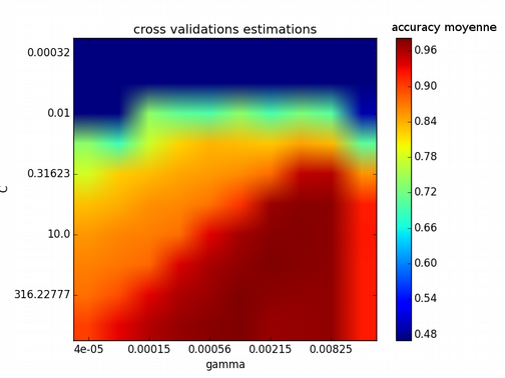
\includegraphics[width=0.5\textwidth]{crossValLog}
  \caption{Scores obtenus pouf 100 validations croisées avec différents couples de paramètres (C,$\gamma$). La couleur d'un point correspond à la précision moyenne de l'algorithme pour le couple (C,$\gamma$) qui lui sert de coordonnées. Les axes sont en échelle logarithmique.}
  \label{fig:crossMap}
\end{figure}

Cette figure montre qu'en effet, la précision de l'algorithme dépend du choix judicieux des méta-paramètres. Le meilleur choix de méta-paramètres dans notre cas est le couple (C,$\gamma$)=(1,$ 10^{-3}$). Nous obtenons alors l'image \ref{fig:veniseSVM} et la matrice de confusion \ref{table:SVC}.

\begin{table}[H]
\begin{center}
 \begin{tabular}{|c|c|c|c|c|}
  \hline
  Nature du terrain & Eau & Champ & Urbain & Rappel \\
  \hline
Eau & 9999 & 0 & 	1 &	100\% \\
Champ & 0 &	9991 &	9 &	99.9\% \\
Urbain &  0 &	244 &	9756 &	97.6\% \\
Précision & 100\% & 97.6\% & 99.9\% & {\color{red}99.1\%} \\
  \hline
  \end{tabular}
\end{center}
\label{table:SVC}
\caption{Matrice de confusion de l'algorithme de Support Vecteur Machine.}
\end{table}

\begin{figure}[H]
  \centering
    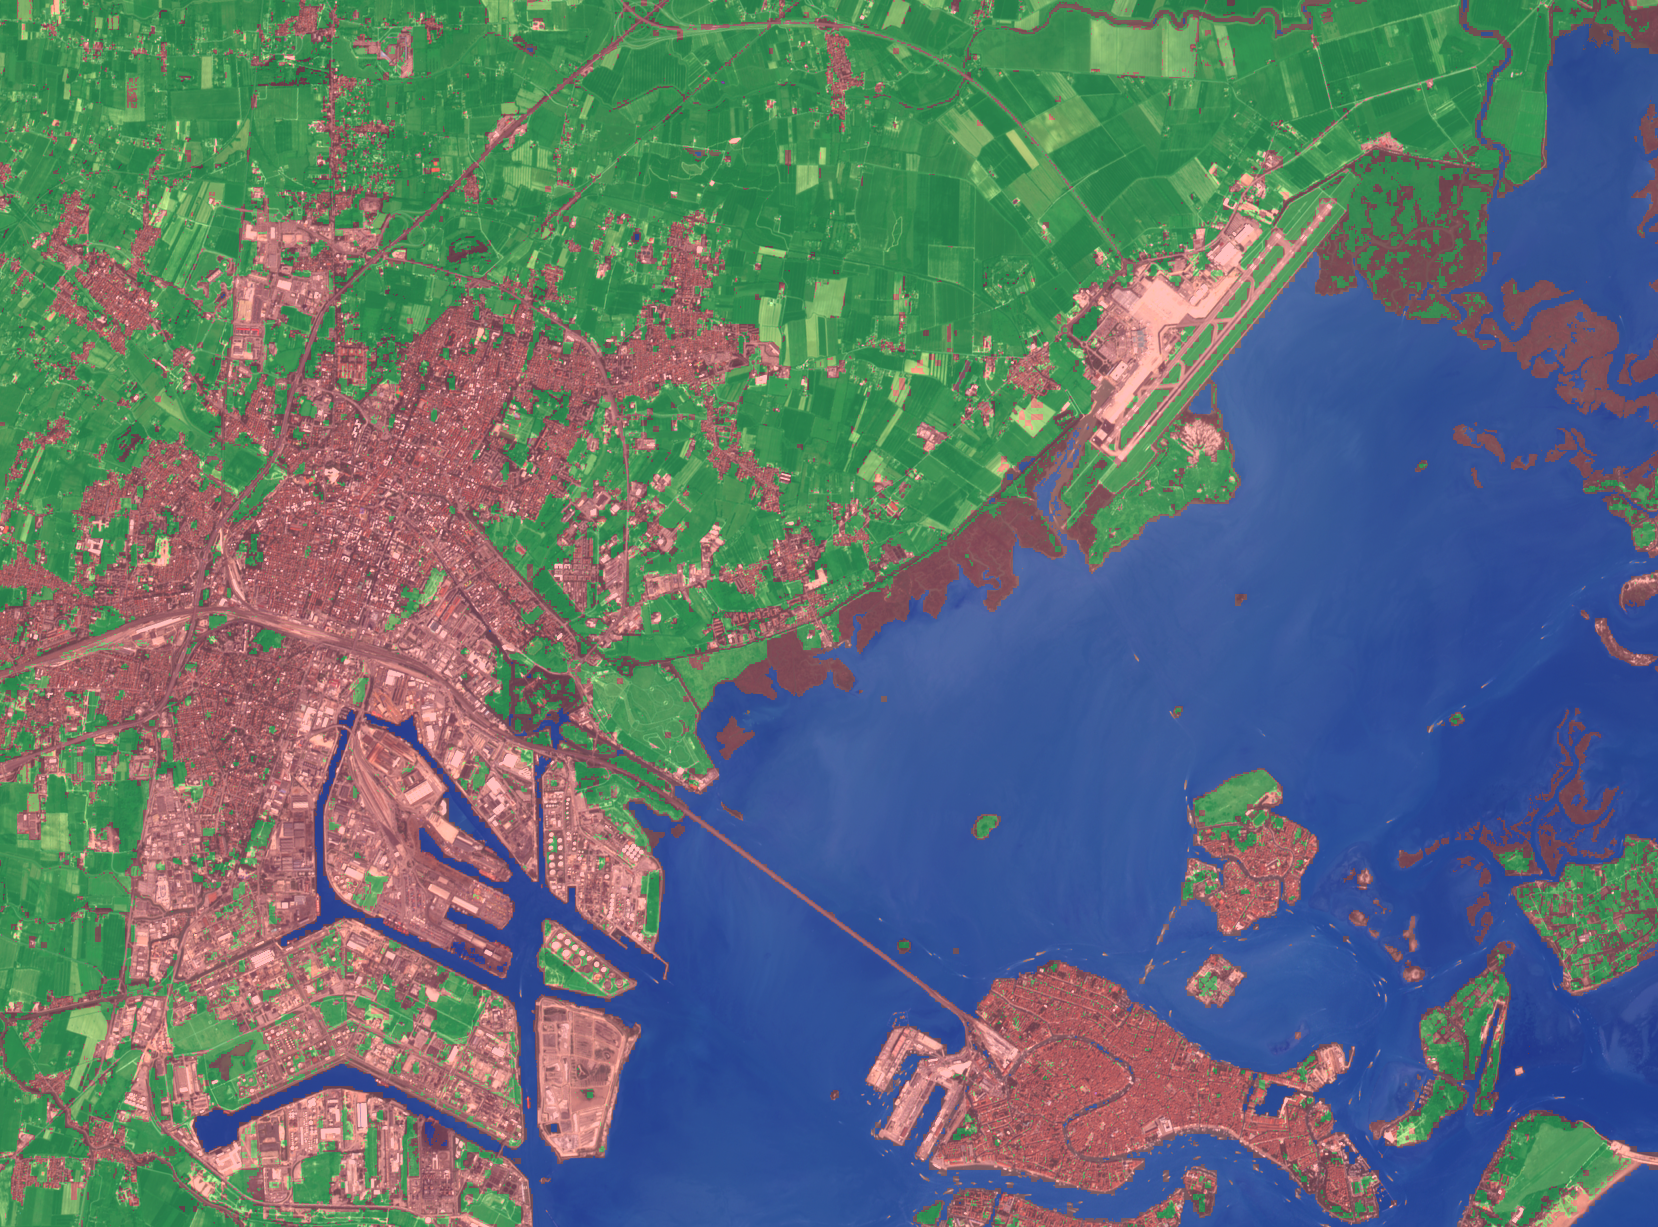
\includegraphics[width=0.75\textwidth]{veniseSVM}
  \caption{Résultat de classification avec le support vecteur machine.}
  \label{fig:veniseSVM}
\end{figure}


\paragraph{Les K plus proches voisins :}

La méthode des k plus proches voisins part d'une idée assez simple. Considérons un ensemble de points, dont les caractéristiques et les classes sont connues. Considérons un nouvel élément à classer. L'idée est qu'il sera de la même classe que le ou les points de caractéristiques les plus proches. Cette méthode présente donc aussi un méta-paramètre : le nombre de voisins k à prendre en compte. 

\begin{figure}[H]
  \centering
    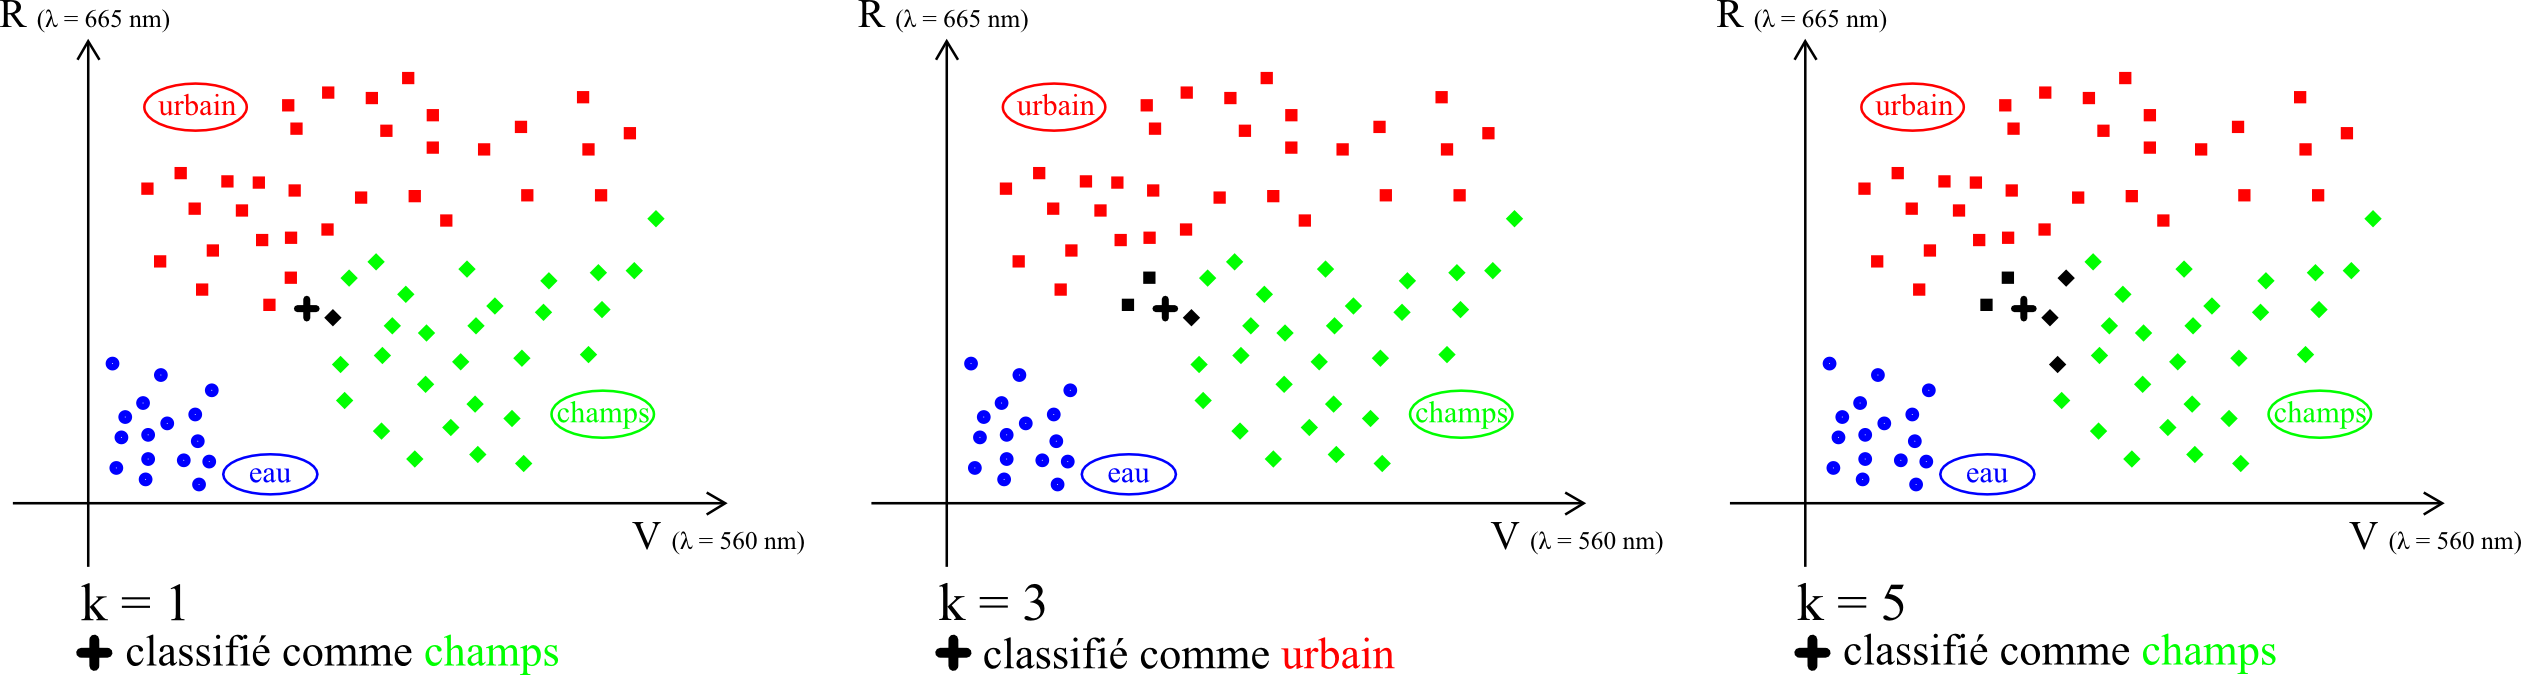
\includegraphics[width=1.1\textwidth]{ml_knn}
  \caption{Classification k plus proches voisins}
  \label{fig:ml_knn}
\end{figure}

Nous avons testé cette méthode avec différentes valeurs de k (1 à 10, 20, 200) et il s'est avéré que les plus faibles valeurs de k sont aussi celles qui fournissent la meilleure exactitude (voir figure \ref{fig:kNN}), ce qui nous laisse penser que les points sont naturellement bien séparés. Nous avons donc choisi de faire notre classification avec la valeur du paramètre k=1. Les résultats obtenus sont montrés sur la figure \ref{fig:1NN} et le tableau \ref{table:1NN}.

La méthode des k-nearest neighbors présente des résultats intéressants, et nous avons obtenu une classification très précise avec cette méthode. 

\begin{table}[H]
\begin{center}
 \begin{tabular}{|c|c|c|c|c|}
  \hline
  Nature du terrain & Eau & Champ  & Urbain & Rappel \\
  \hline
Eau & 9999 & 0 & 	1 &	100\% \\
Champ & 0 &	9929 &	71 &	99.3\% \\
Urbain &  0 &	540 &	9460 &	94.6\% \\
Précision & 100\% & 94.8\% & 99.2\% & {\color{red}98.0\%} \\
  \hline
\end{tabular}
\end{center}
\label{table:1NN}
\caption{Matrice de confusion de l'algorithme de 1-plus proche voisin.}
\end{table}

\begin{figure}[H]
  \centering
    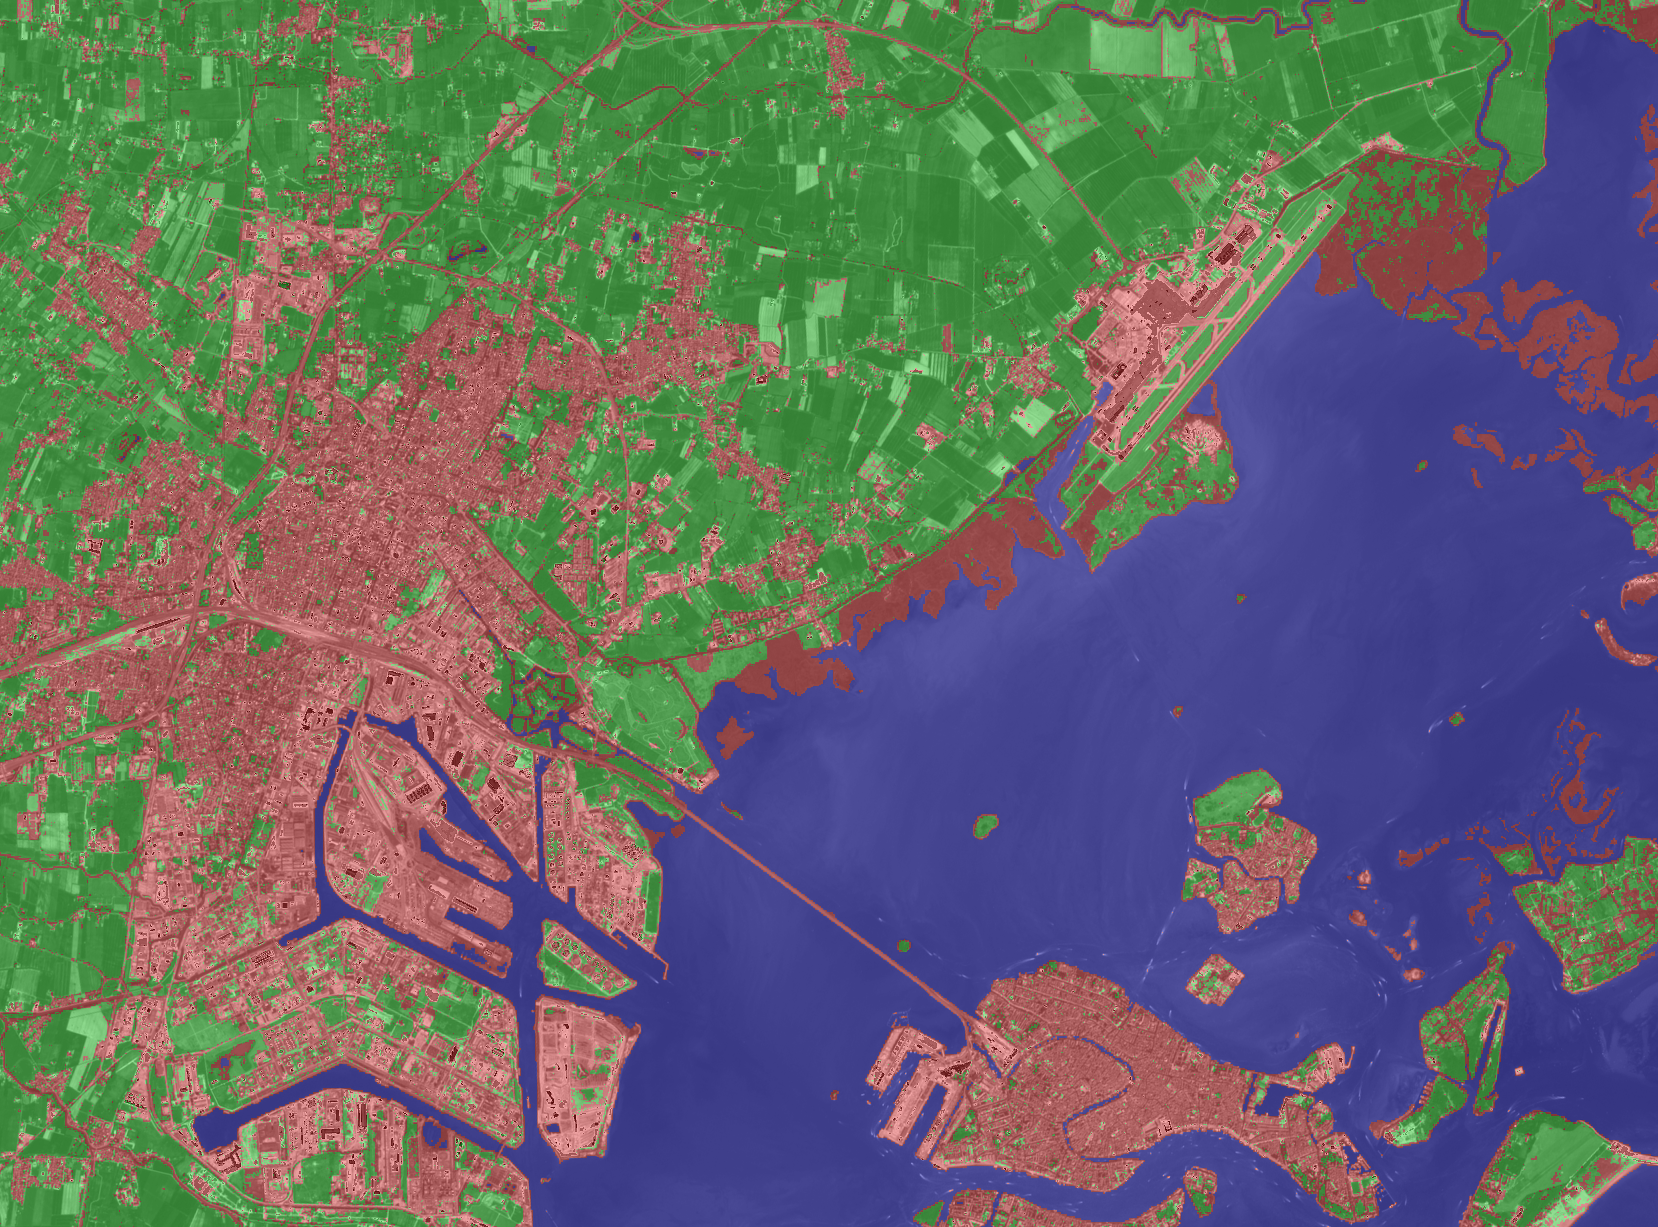
\includegraphics[width=0.75\textwidth]{resultat1NN}
  \caption{Résultat de classification avec la méthode du 1-plus proche voisin}
  \label{fig:1NN}
\end{figure}

On observe également une exactitude en moyenne moindre pour les valeurs paires de k, par rapport aux valeurs impaires : cela vient du fait que nous n'avons pas mis en place de système de vote en cas de conflit. En effet, si la moitié des voisins appartiennent à une classe, et l'autre moitié appartient à une autre classe, le système choisit aléatoirement dans quelle classe placer le pixel. Il est possible de remédier à cela en choisissant un système de vote adapté (par exemple, en cas d'égalité, calculer la distance à chaque voisin et choisir la classe pour laquelle la distance totale est la plus faible).

\begin{figure}[H]
  \centering
    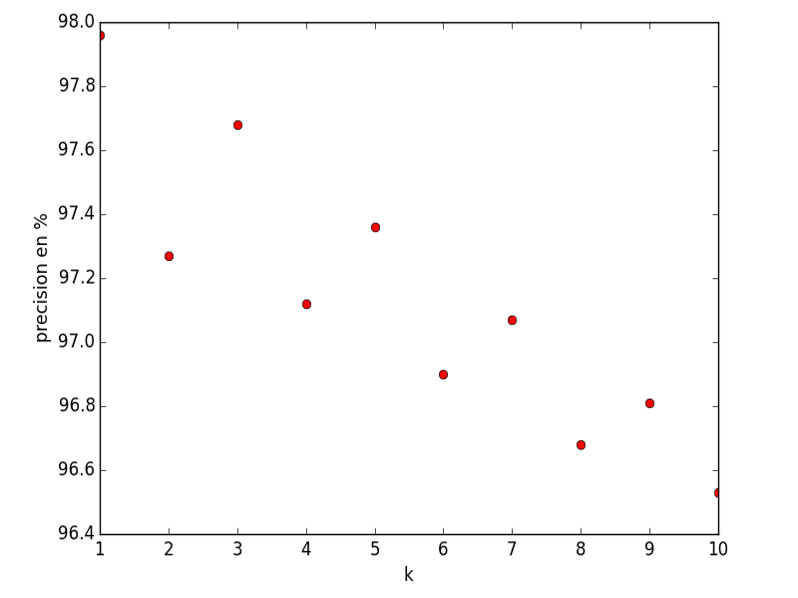
\includegraphics[width=0.5\textwidth]{influencek}
  \caption{Influence du paramètre k sur l'exactitude de l'algorithme.}
  \label{fig:kNN}
\end{figure}

\subsection{Conclusion}
La première conclusion que nous pouvons tirer de notre travail est que les méthodes de machine learning que nous avons testées donnent pour la plupart des résultats très satisfaisants. Le support vecteur machine en particulier nous fournit une exactitude de 98.9\% avec trois classes. Il est d'usage de prétraiter les données pour calculer des indices comme l'index de végétation différentiel normalisé (NDVI)\cite{NDVI}:
\begin{equation}
NDVI=\frac{NIR-VIS}{NIR+VIS}
\end{equation}
Où NIR correspond à l'intensité lumineuse dans le proche infrarouge et VIS dans le rouge. Une valeur de cet indice proche de 1 indique la présence de végétation, une valeur négative indique des nages ou l'absence de végétation. Dans notre cas, les images multispectrales fournissent suffisamment d'informations par elles-mêmes pour classifier les sols avec précision sans passer par cet indice.

L'un des objectifs de notre projet étant de déterminer des principes généraux pour la classification et l'exploitation des données Sentinel-2, nous avons cherché à comparer les résultats obtenus pour différents classificateurs. Nous avons d'abord cherché à comparer à l'œil ces méthodes en cherchant des différences sur les images obtenues, comme sur la figure \ref{comparaison}.

\begin{figure}[H]
  \centering
    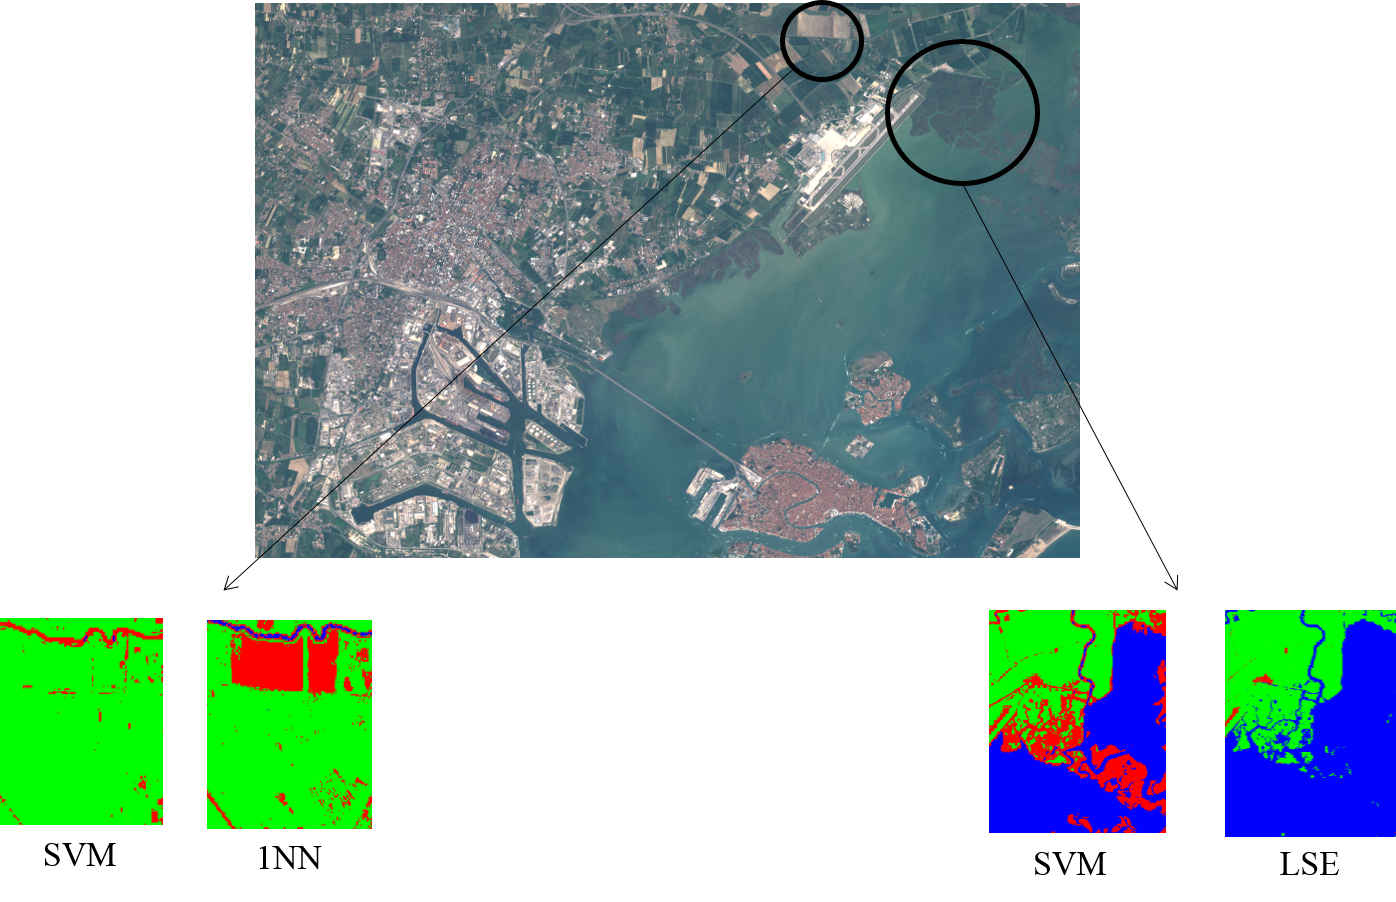
\includegraphics[width=0.75\textwidth]{comparaison}
  \caption{Comparaison des classifications obtenues avec différentes méthodes.}
  \label{fig:comparaison}
\end{figure}
Cependant, ces comparaisons à l'œil ne permettent pas d'identifier formellement un critère meilleur que l'autre. Nous avons donc utilisé un critère numérique : l'exactitude, qui permet de quantifier la qualité de nos classifications et ainsi de les comparer. Les résultats sont résumés dans le tableau \ref{table:comp}. On peut constater que selon ces résultats, le support vecteur machine (SVM) offre les meilleurs résultats et semble donc le classificateur le plus adapté à notre problème de classification à trois classes. Il serait nécessaire de faire des tests similaires sur d'autres zones pour confirmer ou infirmer cette observation, cependant cela sort du cadre de notre projet.

\begin{table}[H]
\begin{center}
 \begin{tabular}{|c|c|c|c|c|}
  \hline
  type de classification & LDA & LSE & 1NN & SVM \\
  \hline
exactitude & 78.4\% & 90.9\% & 	98.0\% & 99.1\% \\
  \hline
  \end{tabular}
\end{center}
\label{table:comp}
\caption{Comparaison des différents classificateurs}
\end{table}

Nous avons également démontré que chacune des 12 bandes spectrales est nécessaire dans la classification, puisque la perte de l'une d'entre elles entraîne une baisse significative de l'exactitude comme on l'a vu dans le paragraphe \ref{lineaire}. Nous avons étudié l'influence de ce paramètre en étudiant l'exactitude d'un classificateur avec les 12 bandes, puis en en retirant. Les résultats obtenus sont présentés en figure \ref{fig:nBandes}.

\begin{figure}[H]
  \centering
    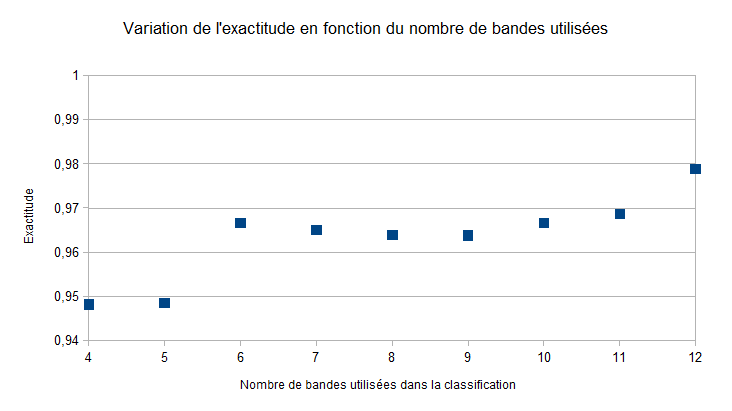
\includegraphics[width=0.5\textwidth]{nb_bands}
  \caption{Influence du nombre de bandes spectrales sur la qualité de classification d'une méthode des 1 plus proches voisins.}
  \label{fig:nBandes}
\end{figure}

\subsection{Limites et améliorations}
Nous avons constaté que la boue le long des côtes n'est pas toujours reconnue de la même manière par nos algorithmes: parfois champs, parfois ville, ils ne correspondent à aucune de nos trois classes. Il est en effet rare en apprentissage automatique d'utiliser seulement trois classes. Nous avons donc rajouté une classe ``boue'' et testé certaines de nos classifications, en particulier le Support Vecteur Machine. Le résultat est donné en figure \ref{fig:SVM4Cl}. La boue est bien classifiée mais l'introduction de cette 4e classe entraîne l'apparition de faux positifs, en particulier dans les champs dont la réponse spectrale est proche.
\begin{figure}[H]
  \centering
    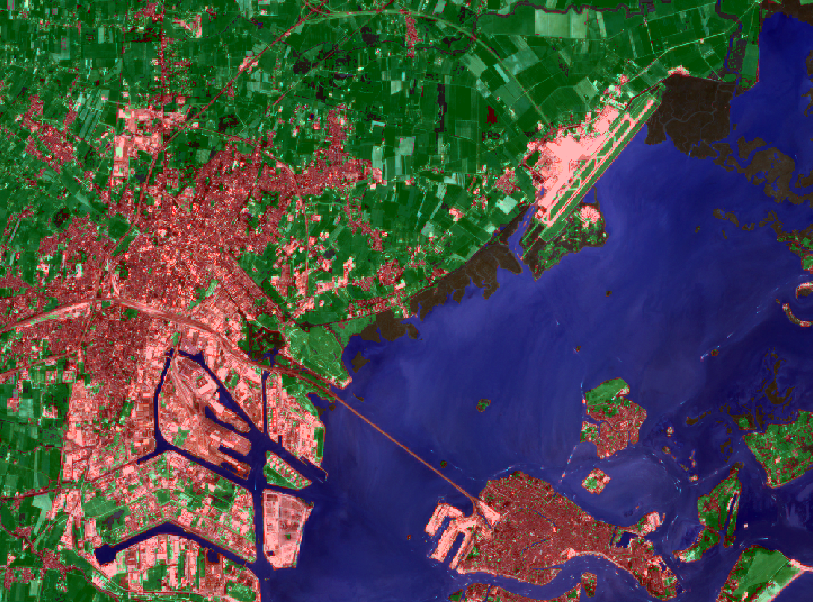
\includegraphics[width=0.75\textwidth]{SVM4Classes}
  \caption{Résultat de classification de 4 classes avec le support vecteur machine.}
  \label{fig:SVM4Cl}
\end{figure}

Plusieurs méthodes s'offrent à nous pour améliorer ce résultat de classification: la plus simple, appelée \textit{whitening} (blanchissement, en français) consiste à centrer chaque bande spectrale sur sa moyenne et à la dilater proportionnellement à son écart-type. Cette méthode renormalise les distributions et permet une meilleure classification.

Il est également possible d'ajouter encore plus d'informations, en utilisant les données de satellites Sentinel-1 qui sont des images radar. Une dernière méthode tout juste mise au point par notre tuteur N. Brodu consiste à améliorer la résolution des bandes spectrales de plus faible résolution en inférant leur valeur à partir des bandes à plus haute résolution. Ces méthodes ont prouvé leur efficacité sur les données MODIS et pourraient apporter un supplément d'information sur les données Sentinel-2 également.

Enfin, les données Sentinel-2 étant toutes nouvelles, peu de zones géographiques sont à notre disposition. Nous nous sommes concentrés pendant ce projet sur une zone précise dans un but de répétabilité. Nous avons essayé de classifier des zones différentes comme présenté en figure \ref{fig:zone2}, cependant ce travail n'a été qu'esquissé et sort du cadre de notre projet.

\begin{figure}[H]
  \centering
    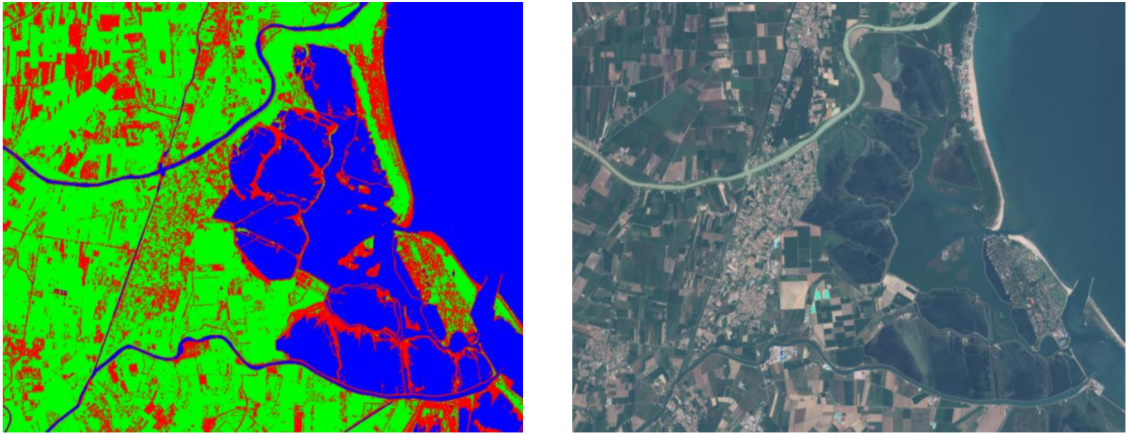
\includegraphics[width=0.7\textwidth]{zone2}
  \caption{Résultat de classification d'une autre zone en Italie du nord}
  \label{fig:zone2}
\end{figure}

Il serait également intéressant d'effectuer un suivi temporel, mais là encore la mission Sentinel-2 est trop récente et les données disponibles ne sont pas suffisantes. 


\bibliography{Biblio}
\bibliographystyle{plain}
\end{document}
